\documentclass{llncs} 

\usepackage[final]{listings}
\usepackage{stmaryrd}
\usepackage{galois}
\usepackage{amssymb}
\usepackage{subfig}
\usepackage{graphicx}


%\newtheorem{theorem}{Theorem}[section]
%\newtheorem{lemma}[theorem]{Lemma}
%\newtheorem{definition}[theorem]{Definition}
%\newtheorem{proposition}[theorem]{Proposition}
%\newenvironment{proof}[1][Proof]{\begin{trivlist}
%\item[\hskip \labelsep {\bfseries #1}]}{\end{trivlist}}

\newenvironment{keywords}{
       \list{}{\advance\topsep by0.35cm\relax\small
       \leftmargin=1cm
       \labelwidth=0.35cm
       \listparindent=0.35cm
       \itemindent\listparindent
       \rightmargin\leftmargin}\item[\hskip\labelsep
                                     \bfseries Key words:]}
{\endlist}


\lstset{language={Java},mathescape=true,flexiblecolumns=true,morekeywords={sealed,case,match,object,def,val,=>},basicstyle=\sffamily\small,moredelim=[is][\itshape]{@}{@},numberstyle=\footnotesize,stepnumber=1,numbersep=2pt}


% This Source Code Form is subject to the terms of the Mozilla Public
% License, v. 2.0. If a copy of the MPL was not distributed with this
% file, You can obtain one at http://mozilla.org/MPL/2.0/.
%
% Copyright (c) 2011-2019 ETH Zurich.

\newcommand{\Sample}{\ensuremath{\mathsf{Sample}}}

\newcommand{\todo}[1]{\textbf{TODO:#1}}
%\newcommand{\todogiulia}[1]{\textbf{TODO GIULIA: #1}}
%\newcommand{\emphgiulia}[1]{\textbf{#1}}
%\newcommand{\emphgiulia}[1]{#1}
%\newcommand{\newpart}[1]{\hl{#1}}
\newcommand{\goodgap}{\hspace{1.536pt}}


\newcommand{\Java}{\ensuremath{\mathsf{Java}}}
\newcommand{\Scala}{\ensuremath{\mathsf{Scala}}}
\newcommand{\CSharp}{\ensuremath{\mathsf{C\#}}}
\newcommand{\FSharp}{\ensuremath{\mathsf{F\#}}}

\newcommand{\lfp}[2]{\ensuremath{\mathit{lfp}^{#1}_{#2} \hspace{2pt}}}
\newcommand{\parts}[1]{\ensuremath{\wp(#1)}}
\newcommand{\dom}[1]{\ensuremath{\cfunction{dom}(#1)}}
\newcommand{\statement}[1]{\ensuremath{\mathtt{#1}}}
\newcommand{\funzione}[2]{\ensuremath{[#1 \rightarrow#2]}}
\newcommand{\pair}[2]{\ensuremath{#1 \times #2}}
\newcommand{\cartesianproduct}[2]{\ensuremath{#1 \times #2}}
\newcommand{\reducedproduct}[2]{\ensuremath{#1 \varotimes #2}}
\newcommand{\true}{\cel{true}}
\newcommand{\false}{\cel{false}}
\newcommand{\booltop}{\cel{\top_B}}
\newcommand{\reducefunction}{\afunction{red}}
\newcommand{\gettype}{\afunction{getType}}
\newcommand{\getstatictype}[1]{\cfunction{\sttype}(#1)}
\newcommand{\sttype}{statictype}
\newcommand{\abstractn}{abstract}
\newcommand{\abstractfunction}[1]{\afunction{\abstractn}(#1)}


\newcommand{\sequence}[1]{\ensuremath{#1^*}}
\newcommand{\sem}[1]{\ensuremath{\llbracket \mathtt{#1} \rrbracket}}
\newcommand{\semanticanome}[1]{\ensuremath{\mathbb{#1}}}
\newcommand{\semantica}[2]{\ensuremath{\semanticanome{#1}\sem{#2}}}

%Concreto

%Dominio e semantica concrete
\newcommand{\cset}[1]{\ensuremath{\mathsf{#1}}}
\newcommand{\ctrace}[1]{\ensuremath{\trace{{\cset{#1}}}}}
\newcommand{\cel}[1]{\ensuremath{\mathsf{#1}}}
\newcommand{\cjoin}{\ensuremath{\cup}}
\newcommand{\cmeet}{\ensuremath{\cap}}
\newcommand{\corder}{\ensuremath{\subseteq}}
\newcommand{\cbot}{\ensuremath{\emptyset}}
\newcommand{\ctop}[1]{\cset{#1}}
\newcommand{\cfunction}[1]{\ensuremath{\mathit{#1}}}
\newcommand{\csemantics}[2]{\ensuremath{\semantica{#1}{#2}}}

%Astratto

%Dominio e semantica astratte
\newcommand{\aset}[1]{\cset{\overline{#1}}}
\newcommand{\ael}[1]{\cel{\overline{#1}}}
\newcommand{\ajoin}{\ensuremath{\sqcup}}
\newcommand{\ameet}{\ensuremath{\sqcap}}
\newcommand{\awidening}{\ensuremath{\nabla}}
\newcommand{\aorder}{\ensuremath{\sqsubseteq}}
\newcommand{\abot}{\ensuremath{\bot}}
\newcommand{\abtop}{\ensuremath{\top}}
\newcommand{\asemantics}[2]{\semantica{\afunction{\semanticanome{#1}}}{#2}}
\newcommand{\atrace}[1]{\ensuremath{\trace{#1}}}
\newcommand{\afunction}[1]{\ensuremath{\overline{\mathit{#1}}}}

%Stringhe
\newcommand{\alphabet}{\ensuremath{\cset{K}}}
\newcommand{\strings}{\ensuremath{\cset{S}}}
\newcommand{\stringlength}[1]{\ensuremath{\cfunction{len}(#1)}}
\newcommand{\charname}{char}
\newcommand{\cchar}[1]{\ensuremath{\cfunction{\charname}(#1)}}

\newcommand{\cstringsemantics}[2]{\ensuremath{\csemantics{\semanticsstatements}{#1}(#2)}}
\newcommand{\cstringsemanticsboolean}[2]{\ensuremath{\csemantics{\semanticsboolean}{#1}(#2)}}
\newcommand{\semanticsstatements}{S}
\newcommand{\semanticsboolean}{B}



\newcommand{\charsinc}{\ensuremath{\cset{\mathcal{CI}}}}
\newcommand{\acharsinc}{\ensuremath{\aset{\charsinc}}}
\newcommand{\acharsinccontains}{\ensuremath{\aset{C}}}
\newcommand{\acharsincmaybe}{\ensuremath{\aset{MC}}}
\newcommand{\acharsincnotcontains}{\ensuremath{\aset{NC}}}
\newcommand{\acharsincsemantics}[2]{\ensuremath{\asemantics{\semanticsstatements_{\charsinc}}}{#1}(#2)}
\newcommand{\acharsincsemanticsboolean}[2]{\ensuremath{\asemantics{\semanticsboolean_{\charsinc}}}{#1}(#2)}

\newcommand{\prefix}{\ensuremath{\cset{\mathcal{PR}}}}
\newcommand{\aprefix}{\ensuremath{\aset{\prefix}}}
\newcommand{\aprefixsemantics}[2]{\ensuremath{\asemantics{\semanticsstatements_{\prefix}}{#1}(#2)}}
\newcommand{\aprefixsemanticsboolean}[2]{\ensuremath{\asemantics{\semanticsboolean_{\prefix}}{#1}(#2)}}

\newcommand{\suffix}{\ensuremath{\cset{\mathcal{SU}}}}
\newcommand{\asuffix}{\ensuremath{\aset{\suffix}}}
\newcommand{\asuffixsemantics}[2]{\ensuremath{\asemantics{\semanticsstatements_{\suffix}}{#1}(#2)}}
\newcommand{\asuffixsemanticsboolean}[2]{\ensuremath{\asemantics{\semanticsboolean_{\suffix}}{#1}(#2)}}

\newcommand{\asinglebrick}{\ensuremath{\aset{\mathcal{B}}}}
\newcommand{\bricks}{\ensuremath{\cset{\mathcal{BR}}}}
\newcommand{\abricks}{\ensuremath{\aset{\bricks}}}
\newcommand{\abrickssemantics}[2]{\ensuremath{\asemantics{\semanticsstatements_{\bricks}}{#1}(#2)}}
\newcommand{\abrickssemanticsboolean}[2]{\ensuremath{\asemantics{\semanticsboolean_{\bricks}}{#1}(#2)}}
\newcommand{\concatlist}{concatList}
\newcommand{\aconcat}[2]{\ensuremath{\afunction{\concatlist}(#1, #2)}}



\newcommand{\stringgraphs}{\ensuremath{\cset{\mathcal{SG}}}}
\newcommand{\astringgraphs}{\ensuremath{\aset{\stringgraphs}}}
\newcommand{\astringgraphssemantics}[2]{\ensuremath{\asemantics{\semanticsstatements_{\stringgraphs}}{#1}(#2)}}
\newcommand{\astringgraphssemanticsboolean}[2]{\ensuremath{\asemantics{\semanticsboolean_{\stringgraphs}}{#1}(#2)}}

\newcommand{\alabel}[1]{\ensuremath{\afunction{lb}(#1)}}
\newcommand{\aoutdegree}[1]{\ensuremath{\afunction{outdegree}(#1)}}
\newcommand{\aroot}[1]{\ensuremath{\afunction{root}(#1)}}
\newcommand{\anormalizebricks}[1]{\ensuremath{\afunction{normBricks}(#1)}}
\newcommand{\anormalizestringgraphs}[1]{\ensuremath{\afunction{normStringGraph}(#1)}}
\newcommand{\apath}[2]{\ensuremath{\afunction{path}(#1,#2)}}

\pagestyle{plain}
\begin{document}
%\title{Debugging and optimizing pattern matching through static type analysis}
\title{Static Type Analysis of Pattern Matching by Abstract Interpretation}

\author{Pietro Ferrara}
\institute{ETH Zurich, Switzerland\\
\email{pietro.ferrara@inf.ethz.ch}}

\maketitle

\begin{abstract}
Pattern matching is one of the most attractive features of functional programming languages. Recently, pattern matching has been applied to programming languages supporting the main current object oriented features. In this paper, we present a static type analysis based on the abstract interpretation framework aimed at proving the exhaustiveness of pattern matchings and the safety of type casts. The analysis is composed by two distinct abstract domains. The first domain collects information about dynamic typing, while the second one tracks the types that an object cannot be instance of. The analysis has been implemented and applied to all the \Scala\ library. The experimental results underline that our approach scales up since it analyzes a method in 90 msec in average. In addition, the analysis is precise in practice as well, since we prove the exhaustiveness of 42\% of pattern matchings and 27\% of the type casts without any manual annotation on the code.
\end{abstract}
\begin{keywords}
Abstract interpretation, static analysis, pattern matching.
\end{keywords}

\section{Introduction}
Pattern matching is recognized to be one of the most expressive features of functional programming languages. Extending its full expressiveness to programming languages supporting the current object oriented features is not straightforward \cite{EMI07}. In fact, features like inheritance and information hiding are not supported by the functional pattern matching, since it dealt with algebraic data types. Nevertheless, recent work \cite{EOW07,SNM07} introduced pattern matching in programming languages supporting the main current object oriented features as \FSharp\ \cite{FSharp} and \Scala\ \cite{Scala}. In addition, some extensions of \Java\ supporting pattern matching appeared in the last few years \cite{HNB08,RL07}. Pattern matching checks if an expression respects a given pattern looking at an ordered list of case expressions. One of the most common case expressions is the type case: we select the case to apply following the dynamic type of the expression. Consider the \Scala\ program in Figure \ref{fig:typecases}. The content of argument \statement{x} is matched with respect to its type: if it is an instance of \statement{Something}, the method returns the string representing the contained value. Otherwise, the type of \statement{x} is \statement{None}, and  \statement{extract} returns the empty string.

Languages like \FSharp\ and \Scala\ are compiled into a bytecode language (for instance, MSIL \cite{ECMA06} or \Java\ bytecode \cite{JVMspecification}) that supports the main imperative features. Thus type cases in pattern matching are translated into type tests and casts. For instance, the body of method \statement{extract} in Figure \ref{fig:typecases} is translated into the code in Figure \ref{fig:runningexample} by the \Scala\ compiler \cite{EMO07}. Note that information about generics is erased.
\begin{figure}
\centering
\begin{lstlisting}
abstract sealed class Option[T]
final case class Something[T](val y : T) extends Option[T]
final case object None extends Option[Nothing]

def extract[T](x : Option[T]) : String = x match {
  case Something(y) => return y.toString();
  case None => return ""; 
}
\end{lstlisting}
\caption{Pattern matching with type cases}
\label{fig:typecases}
\end{figure}
\begin{figure}
\centering
\begin{lstlisting}[numbers=left, numberstyle=\tiny]
String extract(Option x) {
	if(x instanceOf Something)
		return ((Something) x).y.toString();
	else if (x instanceOf None)
			return "";
		else throw new MatchError (); 
}
\end{lstlisting}
\caption{Results of \Scala\ compilation}
\label{fig:runningexample}
\end{figure}
This code can be easily optimized adopting a specific static analysis. When \statement{x\ instanceof\ Something} is false, we know that \statement{x\ instanceof\ None} is always true. In fact, the static type of \statement{x} is \statement{Option}, this class is \statement{abstract}, and the only two classes that extend it are \statement{Something} and \statement{None}. Note that \statement{Option} is declared as \statement{sealed}. In \Scala, a \statement{sealed} class can be extended only by classes that are defined in the same source file. Therefore we know that \statement{Option} cannot be extended by external code, and we can conclude that the \statement{if} statement at line \statement{4} is always evaluated to \statement{true}. In addition, we know that the statement \statement{throw\ new\ MatchError()} is unreachable, that is the pattern matching contained by the original \Scala\ program is exhaustive. Finally, the type cast at line \statement{3} is safe.

\subsection{Contribution}
\begin{figure}
\centering
\subfloat[Type hierarchy]
{
\centering
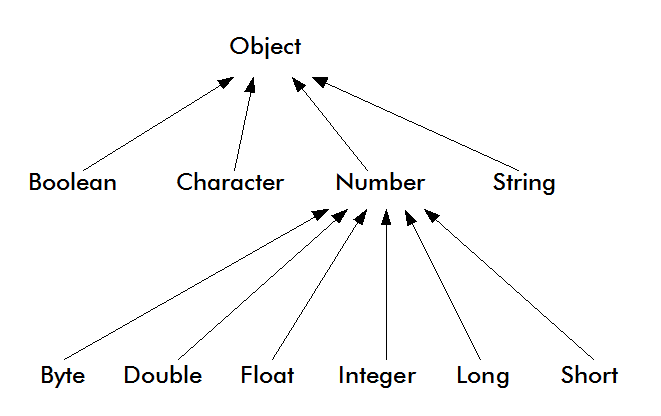
\includegraphics[width=5.5cm]{type_system.png}
\label{pict:type}
} \qquad
\subfloat[Static typing]
{
\centering
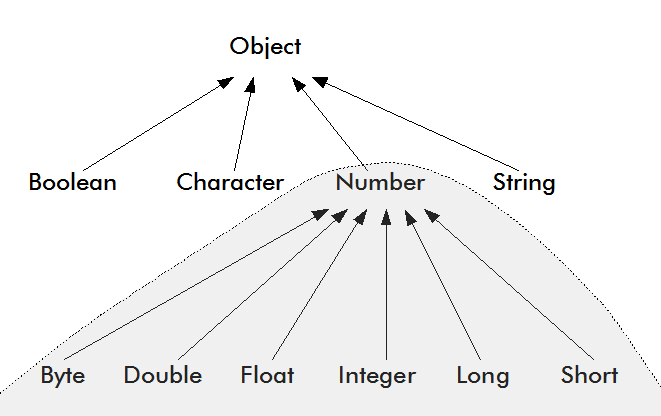
\includegraphics[width=5.5cm]{static_typing.png}
\label{pict:statictype}
}\\
\subfloat[Dynamic typing \dynamictype]
{
\centering
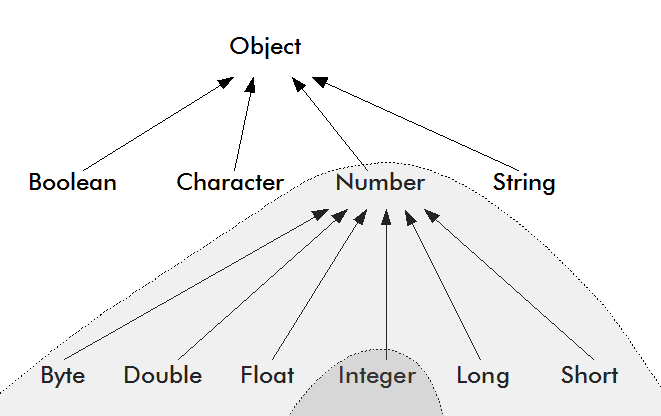
\includegraphics[width=5.5cm]{dynamic_typing.png}
\label{pict:dynamictype}
} \qquad
\subfloat[Not-instance-of domain \nottype]
{
\centering
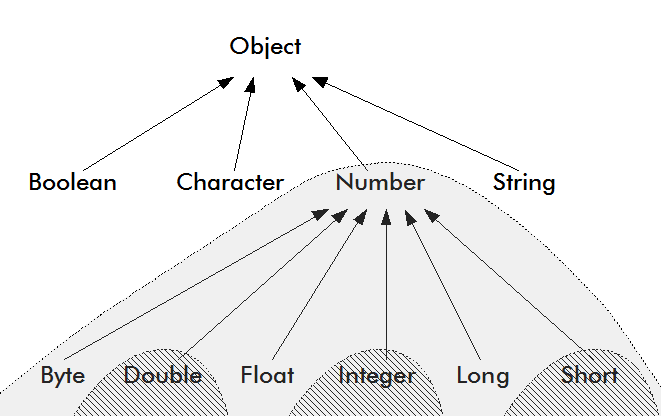
\includegraphics[width=5.5cm]{not_typing.png}
\label{pict:nottype}
}\\
\caption{Type system and abstract domains}
\end{figure}

The main contribution of this paper is the introduction of two new abstract domains in order to capture precise information on the types of variables. The two main goals of our analysis are precision and efficiency. Precision is achieved through the development of abstract domains focused on the properties of interest, that is, exhaustiveness of pattern matching and safety of casts. Efficiency is achieved through a modular analysis. For this reason, our approach is based on the Design-by-Contract (DbC) methodology \cite{meyer97}. This means that when we analyze a method call we rely on class invariants, pre and post conditions. Thanks to this approach, we do not need to analyze the whole program, but we can analyze a method alone relying on its contracts. In a similar way, we rely on language constructs like \statement{sealed} in \Scala\ in order to be sure that a class cannot be extended by external code.

In this paper, we do not deal with issues related to the heap and its analysis. Hence the language on which we are going to define our analysis does not contain field accesses, aliasing, etc., but it deals only with variables. The object oriented programs we analyzed are preprocessed by a sound heap analysis that replaces heap accesses with variables. This means that method calls may have side effects on these variables. The heap analysis we perform is quite rough: intuitively, we approximate all the instances of the same class with the same variable, and we perform weak updates \cite{CWZ90} as these abstract references may represent several concrete references. Then the number of abstract references is bounded to the number of classes of the analyzed program. In this way we preserve the scalability of our approach. On the other hand, it may seem that this approach is too much coarse since we approximate all the fields having the same static type with the same variable. Indeed, this does not particularly affect the precision of our approach because, for the most part of the programs we analyzed, the content of fields is first stored in a local variable (and in this way we obtain a specific variable identifier), and then type checking and casts are performed on this local variable.

Consider now the type hierarchy depicted in Figure \ref{pict:type}. The class \statement{Object} is extended by several subclasses that represent different types in a programming language, e.g., \statement{Boolean}. The abstract class \statement{Number} is extended by several subclasses, each representing one possible numerical type, e.g., \statement{Integer}. For instance, Figure \ref{pict:statictype} represents a situation in which the static type of a variable is \statement{Number}. The static type information guarantees that the objects assigned to a variable are instances of its static type or of one of its subclasses. Thus instances of \statement{Long}, \statement{Float}, etc. may be assigned to a variable whose static type is \statement{Number}.

The first abstract domain we are going to define is \dynamictype. It is aimed at approximating information about the dynamic type of variables. Figure \ref{pict:dynamictype} depicts a case in which we assign an object instance of the \statement{Integer} class (darker area) to a variable of static type \statement{Number} (light grey area). The information about dynamic typing comes mainly from assignments, type casts, \statement{new} statement, and assumption of \statement{instanceof} conditions. Since we rely on DbC, if a method has no postcondition about the dynamic type of variables (e.g., the returned value), we would abstract its type information using its static type after the method call.

The second domain we are going to define is \nottype. It abstracts the types that a variable cannot be instance of. For instance, Figure \ref{pict:nottype} depicts a situation in which a variable of static type \statement{Number} cannot be instance of \statement{Double}, \statement{Integer}, or \statement{Short}. In this way we can discard some leaves of the type tree. This information is collected when we assume the negation of an \statement{instanceof} boolean condition. We could have adopted a different approach capturing a set of types for each variable representing all the possible types a variable can have at a given program point. In this way, we may model that an object cannot be instance of a type simply removing the type from the set of types related to it. Unluckily this solution is not feasible for two main reasons. Imagine to be after a method call, where we know only the static type of a variable. In this context, assuming that an object cannot be instance of a given type (i) may affect the performance (e.g., if its static type is \statement{Object} and we have to exclude \statement{String} we should relate the variable to a set of types of huge dimensions), (ii) cannot be represented since our analysis is modular and external code usually defines and instantiates new classes. One may argue that, since we are interested in proving the exhaustiveness of pattern matching, we can restrict the analysis only on types that cannot be extended by external code. With such restriction the approach based on set of possible types would be feasible, and performance could be preserved supposing that we have few subclasses. First of all, we want to track information also on classes that can be externally extended, in order to eventually provide information to developers like \textquotedblleft if this class would be \statement{sealed}, then the pattern matching would be exhaustive\textquotedblright. This solution would not collect the information necessary to provide this output. In addition, we do not expect in general that \statement{sealed} classes (or more generally classes that cannot be extended by external code) have only few subclasses, since each subclass may be used to represent a particular case of a complex data structure.
%(ii) we do not think that classes involved have always few subclasses, since pattern matching sometimes inspect complex structures (for instance, the expressions of a programming language, where each distinct type of expression is encoding using a distinct class).

Combining $\dynamictype$ and $\nottype$, we are in position to obtain precise information about types and prove the safety of some cast operations, and the unreachability of some code, in particular when dealing with pattern matching.

The analysis works on a simple object oriented language. We designed it in order to translate the main object oriented programming languages into this language. In this way, we want to apply our analysis to several languages. Up to now, we have developed the translation of the \Scala\ programming language. Thus our analysis is focused on the code obtained from the \Scala\ pattern matching statements. In this context, if we prove that a \statement{MatchError} exception is unreachable, this means that the pattern matching is exhaustive.

The analysis has been implemented and the experimental results underline that our approach scales up. We are in position to analyze \Scala\ libraries (more than 30.000 methods) in less than one hour, and in average we require 90 milliseconds to analyze a single method. In addition, it turns out that the analysis is precise in practice. In fact, we are able to prove the exhaustiveness of 42\% of pattern matchings (that may contain not only type cases but also other cases whose information is not captured by our analysis) and 27\% of the type casts without any manual annotation of the code.

The following of this section introduces some preliminaries on abstract interpretation. Section \ref{sect:language} presents the language that we analyze. Section \ref{sect:concrete} introduces the concrete domain and semantics, while Section \ref{sect:domain} formalizes the two domains adopted by our analysis, and explains how they work on an example. Section \ref{sect:experimentalresults} presents the experimental results, and Section \ref{sect:relatedwork} introduces the related work. Finally, Section \ref{sect:conclusion} concludes and discusses the future work.

\subsection{Abstract Interpretation}
Our approach is based on abstract interpretation \cite{CC77,CC79}, a theory for defining and soundly approximating the semantics of a program. A concrete semantics, aimed at specifying the runtime properties of interest, is defined. Then it is approximated to obtain an abstract semantics computable but still precise enough to capture the property of interest, and specified by an abstract domain and an abstract transition function.

Formally, the concrete domain $\cset{D}$ is a lattice $\langle \cset{D}, \sqsubseteq_\cel{C}, \bot_\cel{C}, \top_\cel{C}, \sqcup_\cel{C}, \sqcap_\cel{C} \rangle$. The concrete elements are related to the abstract domain $\langle \aset{D}, \aorder_\cel{A}, \abot_\cel{A}, \abtop_\cel{A}, \ajoin_\cel{A}, \ameet_\cel{A} \rangle$ by a concretization function $\gamma$ and an abstraction function $\alpha$. In order to obtain a sound analysis, we require that they form a Galois connection; we denote it by  $\langle \cset{D}, \sqsubseteq_\cel{C}, \bot_\cel{C}, \top_\cel{C}, \sqcup_\cel{C}, \sqcap_\cel{C} \rangle \galois{\alpha}{\gamma} \langle \aset{D}, \aorder_\cel{A}, \abot_\cel{A}, \abtop_\cel{A}, \ajoin_\cel{A}, \ameet_\cel{A} \rangle$.

A semantics is defined on the abstract and concrete domains. Given a state of the domain and a statement, it produces the result of the execution of the statement starting from the given state. The abstract semantics $\afunction{\semanticanome{S}}$ has to soundly approximate the concrete one, that is $\forall \ael{d} \in \aset{D} : \csemantics{S}{\gamma(\ael{d})} \sqsubseteq_\cel{A} \gamma \circ \asemantics{S}{\ael{d}}$. Usually, the semantics is defined as the computation of a fixpoint \cite{CC79}.

Different domains can be combined in Cartesian products. Let $\cartesianproduct{\aset{A}}{\aset{B}}$ be the Cartesian product of abstract domains $\aset{A}$ and $\aset{B}$. The lattice operators are defined as the pointwise application on the components of the pairs of the lattice operator on each abstract domain. The reduced product $\reducedproduct{\aset{A}}{\aset{B}}$ is a Cartesian product on which a $\cfunction{reduce}$ function is provided: given a state of the Cartesian product, it mutually refines the information contained in each domain using the information provided by the other domain.
\subsubsection{Generic analyzers}
Abstract interpretation can be applied in order to develop generic analyzers \cite{COU99}. In particular, this theory allows one to define a compositional analysis, e.g., an analysis that can be instantiated with different numerical domains, and in order to analyze different properties. Many different generic analyzers have been proposed recently \cite{FER09a,LF08,SPO05}. The type analysis we present in this paper has been implemented in \analyzer\ (Static Analyzer of Multiple Programming LanguagEs). This generic analyzer can be plugged with different numerical domains and heap analysis. In addition, it can be extended with new analyses like our type analysis.

\section{Language}

\label{sect:language}


\begin{table}[t]
\begin{center}
\begin{tabular}{llr|llr|llr}
\statement{C ::=} & \statement{x = E} & (C1) & \statement{E ::=} & \statement{new\ T()} & (E1) & \statement{B ::=} & \statement{x\ instanceof\ T} & (B1)\\
& \statement{declare\ x\ :\ T} & (C2) & & \statement{x} & (E2) & & \statement{!\ x\ instanceof\ T} & (B2)\\
& \statement{assume(B)} & (C3) & & \statement{(T)\ x} & (E3) & & & \\
& \statement{x.M(y1, ..., yn)} & (C4) & & & & & &\\
\end{tabular}
\end{center}
\caption{OO core language}
\label{fig:language}
\end{table}

We introduce a core language in order to make explicit the main characteristics of our abstract domains. It consists of assignments (C1), declarations of variables (C2), assumptions of boolean conditions (C3), and method calls (C4). An expression that can be assigned to a variable is the instantiation of a class (E1), another variable (E2), or the cast of a variable (E3). A condition can be the check that the dynamic type is instance of (B1) or it is not instance of (B2) a type.

We focus our attention only on the main aspects of the type analysis we are interested in, that is, casts and runtime checks of dynamic types. Nevertheless, our implementation covers all the features of current programming languages, as numerical operations, field accesses, etc. Intuitively, we represent the body of a method through a Control Flow Graph (CFG). Each block in the CFG contains a list of statements. Different blocks are connected through edges that could eventually contain a boolean condition to represent conditional jumps. In this way, we support control structures like \statement{if} statements and \statement{while} loops.

\section{Concrete Domain and Collecting Semantics}
\label{sect:concrete}
The concrete domain is composed by environments that collect the dynamic type for each variable. Formally, $\cset{Env} : \funzione{\variables}{\types}$. The concrete domain is composed by sets of environments. Each environment represents one possible execution of the program in a given point. The lattice is obtained using set operators. Formally, $\langle \parts{\cset{Env}}, \subseteq, \cup, \cap, \cset{Env}, \emptyset \rangle$. 

We define the collecting semantics as a function that, given an environment and a statement, returns the environment resulting from the execution of the given statement on the given environment.  Table \ref{fig:collectingsemantics} reports the formal definition of this collecting semantics\footnote{$\cfunction{execute}(\statement{x.M(y1, ..., yn)}, \cel{d})$ resolves and executes method \statement{M} on \cel{d}}. $\aorder_{\types}$ corresponds to the subtype relation, while $\bot$ is used to represent a situation in which the execution is stopped because of an unsafe dynamic cast. The collecting semantics is aimed at formalizing the runtime behaviors focusing on the information we are interested. The extension of this semantics to our concrete domain (that is made by set of environments) is the application of this semantics on each environment in the initial state.

$\cfunction{\semanticanome{S}}$ is the basic step adopted in order to compute the semantics of a method on its CFG representation. Intuitively, we build up incrementally the traces representing the executions of a method relying on $\cfunction{\semanticanome{S}}$ to perform single computational steps \cite{COU02}. Since non-deterministic behaviors are possible (e.g., because of inputs from the user) and these may also affect the type information, we consider sets of traces.

\begin{table}[t]
\begin{center}
\begin{tabular}{l|l|l}
$\csemantics{E}{\statement{new\ T()}, \cel{d}}=\statement{T}$ & 
$\csemantics{B}{\statement{x\ instanceof\ T}, \cel{d}}=$ &
$\csemantics{S}{\statement{x = E}, \cel{d}}=\cel{d}[\statement{x} \mapsto \csemantics{E}{\statement{E}, \cel{d}}]$\\

$\csemantics{E}{\statement{x}, \cel{d}}=\cel{d}(\statement{x})$ &
\hspace{10pt} $=\cel{d}(\statement{x}) \aorder_{\types} \statement{T}$ &
$\csemantics{S}{\statement{declare\ x\ :\ T}, \cel{d}}=\cel{d}[\statement{x} \mapsto \statement{T}]$\\


$\csemantics{E}{\statement{(T)\ x}, \cel{d}}=$ &
$\csemantics{B}{\statement{! B}, \cel{d}} = \neg \csemantics{B}{\statement{B}, \cel{d}}$& 
$\csemantics{S}{\statement{assume(B)}, \cel{d}}=$\\

\hspace{10pt} $=\left\{
\begin{array}{ll}
\cel{d}(\statement{x}) & \textrm{ if } \cel{d}(\statement{x}) \aorder_{\types} \statement{T}\\
\bot & \textrm{ otherwise}\\
\end{array}
\right.$&
&
\hspace{10pt} $=\left\{
\begin{array}{ll}
\bot & \textrm{ if } \csemantics{B}{\statement{B}, \cel{d}}=\false\\
\cel{d} & \textrm{ if } \csemantics{B}{\statement{B}, \cel{d}}=\true\\
\end{array}
\right.$
\\

&
&
$\csemantics{S}{\statement{x.M(y1, ..., yn)}, \cel{d}}=$\\

&
&
\hspace{10pt} $=\cfunction{execute}(\statement{x.M(y1, ..., yn)}, \cel{d})$\\
\end{tabular}
\end{center}
\caption{Collecting semantics}
\label{fig:collectingsemantics}
\end{table}


\section{Abstract Domain and Semantics}
\label{sect:domain}

In this section, we present and formalize the two abstract domains of our analysis, how we combine them, and we explain how they work in practice on the example presented in Figure \ref{fig:runningexample}. Note that we will define the abstract semantics only on single statements. Its extension to blocks and CFGs is obtained as usual in approaches based on abstract interpretation and trace semantics relying on the upper bound operators \cite{CC77}.

\subsection{Static Typing}

The programming language introduced in Section \ref{sect:language} provides some information on the static types of variables. We suppose that a subtype relation $\aorder_{\types}$ is provided, and that this is a partial ordering. Given two types $\ael{t}_1, \ael{t}_2 \in \types$, $\ael{t}_1 \aorder_{\types} \ael{t}_2$ if and only if $\ael{t}_1$ is subtype of $\ael{t}_2$. We denote by $\ajoin_{\types}$ and $\ameet_{\types}$ respectively the upper and lower bound operators univocally identified by $\aorder_{\types}$. These operators form a lattice. In this way, we support the most part of common object oriented type systems \cite{CAR04}, like the ones of \Java, \CSharp, \Scala, and \FSharp.
%The type structure can be represented as a lattice of finite height. We suppose this information is provided. Thus we suppose that the typing lattice $\langle \types, \aorder_{\types}, \ajoin_{\types}, \ameet_{\types}, \abtop_{\types}, \abot_{\types} \rangle$ is provided. In object oriented languages, the ordering operator is the subtyping relation. The supposition that the type hierarchy has a lattice structure is not restrictive, as it allows the most expressive features of object oriented programming languages like multiple inheritance \cite{CAR04}. 

Each type represents itself and all the types that are its subtype. Note that this is exactly the semantics of a static type: at runtime a variable of static type \ael{t} can have a type that is \ael{t} or one of its subtypes. Formally, the concretization of a type \ael{t} is defined as $\gamma_{\types}(\ael{t})=\{\ael{t'} : \ael{t'} \aorder_{\types} \ael{t}\}$. Since information about static typing can be considered as syntactic sugar, we suppose that a function $\cfunction{\sttype} : \funzione{\variables}{\types}$ is provided. Given a variable, it returns its static type.

%\textbf{Semantics } We will define the semantics only on the statements that change the state of the \statictype\ domain.
%\[
%\begin{array}{l}
%\asemanticsstatictyping{\statement{declare\ x\ :\ T}, \ael{st}}=\ael{st}[\statement{x} \mapsto \statement{T}]\\
%\asemanticsstatictyping{\statement{x.M(y1, ..., yn)}, \ael{st}}=\ael{st}\\
%\end{array}
%\]
%Intuitively, our static typing domain tracks information only when a variable is declared. Note that a method call would not change the information contained in the \statictype\ domain. In fact, the information about static typing is preserved after a method call. Even if the method may have side effects on variables (since these may represent heap locations because of the preprocessing phase operated by the heap analysis), it has to respect their static types.\\
%\textbf{Running example } Suppose to analyze method \statement{extract} of the example presented in figure \ref{fig:runningexample}. From the declaration of the arguments of the method, we know that at the beginning of the method the state of our static type domain is $[\statement{x} \mapsto \statement{Option}]$. After the computation of the semantics of the method, we would still obtain this state at each program point, as we do not declare any new variable. Note that using this domain we are not able to check that the cast at line \statement{3} is safe, nor that line \statement{5} is unreachable.


\subsection{\dynamictype: Dynamic Typing}

\dynamictype\ abstracts the dynamic type of variables. 
%While the static typing considers the type of variables when they are declared, this domain over-approximates the dynamic type of variables. Type-safe languages guarantee that we can assign to a variable only objects that are instances of its static type or of one of its subtypes. Thus the information collected by this domain is more precise than the static type domain. Note that when a method is called, the information about dynamic types may be not preserved because of side effects, while the one about static typing is preserved.
Relying on \types\ we build up the domain $\dynamictype : \funzione{\variables}{\types}$ that relates each variable to its dynamic type. The operators on the lattice $\langle \dynamictype, \aorder_{\dynamictype}, \ajoin_{\dynamictype}, \ameet_{\dynamictype}, \abtop_{\dynamictype}, \abot_{\dynamictype} \rangle$ are obtained as the functional extension of the ones of \types. The information inferred by \dynamictype\ is refined with the static type information provided by the $\cfunction{\sttype}$ function: if the type of a variable $\statement{v}$ is not yet defined, the dynamic type domain returns its static type, that is, $\getstatictype{\statement{v}}$. The concretization of $\dynamictype$ is defined as the functional extension of $\gamma_{\types}$ as well. Formally, $\gamma_{\dynamictype}(\ael{f})=\{[\statement{v} \mapsto \ael{t}] : \statement{v} \in \dom{\ael{f}} \land \ael{t} \in \gamma_{\types}(\ael{f}(\statement{v}))\}$.

\subsubsection{Semantics}
\[
\begin{array}{l}
\asemanticsdynamictyping{\statement{x=y}, \ael{dt}}=\ael{dt}[\statement{x} \mapsto \ael{dt}(\statement{y})]\\
\asemanticsdynamictyping{\statement{x=new\ T()}, \ael{dt}}=\ael{dt}[\statement{x} \mapsto \statement{T}]\\
\asemanticsdynamictyping{\statement{x=(T) y}, \ael{dt}}=\ael{dt}[\statement{x} \mapsto \statement{T} \sqcap_\types \ael{dt}(\statement{y}), \statement{y} \mapsto \statement{T} \sqcap_\types \ael{dt}(\statement{y})]\\
\asemanticsdynamictyping{\statement{assume(x\ instanceof\ T)}, \ael{dt}}=\ael{dt}[\statement{x} \mapsto \ael{dt}(\statement{x}) \ameet_\types \statement{T}]\\
\asemanticsdynamictyping{\statement{x.M(y1, ..., yn)}, \ael{dt}}=\asemanticsdynamictyping{\statement{assume(rename(postcondition_M))}, \abtop_{\dynamictype}}\\
\end{array}
\]
%What is different w.r.t. \statictype\ is the semantics. In particular, while \statictype\ was interested in variable declarations, \dynamictype\ deals with assignment to variables and checking of conditions.
When a variable is assigned to another one (\statement{x=y}), we capture that the dynamic type of \statement{x} is the type of \statement{y}. Similarly, when we assign to a variable the instance of a fresh object, we relate this variable to the type of the new object. The dynamic type of the assignment of a cast to type \statement{T} of a variable \statement{y} is the lower bound between the dynamic type of \statement{y} and type \statement{T}. Thus, it may be the case in which it contains a type that is more approximated than \statement{T}\ even if the cast is safe. After the cast, we know that its dynamic type will be surely \statement{T} or one of its subtypes. This is why we take the lower bound between the dynamic type of the variable and \statement{T}.  In a similar way, when we test to \statement{true} a boolean condition like \statement{x\ instanceof\ T}, we track that the dynamic type of \statement{x} is the lower bound of its type and \statement{T}. When we analyze a method call, we assume the postconditions of this method call, that may contain some type information, on the top state of the \dynamictype\ domain. Since we do not consider framing information, we suppose that potentially a method may access and assign all the variables of the current state of computation. Then we assume the postcondition on a top state in order to preserve the soundness of our analysis. In addition, we suppose that a \statement{rename} function is provided, and it renames all the variables contained in the postcondition matching the calling environment.

\subsubsection{Running Example}
At the beginning of the analysis of method \statement{extract} we have no information about dynamic typing, but we know that the static type of \statement{x} is \statement{Option}. When we analyze the condition of the \statement{if} branch at line \statement{2} we calculate that the state leading to the \statement{then} statement of our dynamic type domain is $[\statement{x} \mapsto \statement{Something}]$, since the condition is evaluated to \true. In the same way, at line \statement{4} we obtain that $[\statement{x} \mapsto \statement{None}]$. Thus we prove that the cast at line \statement{3} is safe, while we are not able yet to detect that line \statement{6} is unreachable.


%\subsection{\staticdynamictype: Cartesian product of \statictype\ and \dynamictype}
%
%As already explained, usually the information abstracted by \dynamictype\ is more precise than the information contained in \statictype. On the other hand, when a method is called, following the DbC approach we lose all the information about dynamic typing, and in this case \statictype\ is more precise than \dynamictype. When we ask what is the type of a variable, we want to obtain the most precise type.
%
%We consider the Cartesian product of these domains $\staticdynamictype=\cartesianproduct{\statictype}{\dynamictype}$. The lattice operators of $\langle \staticdynamictype, \aorder_{\staticdynamictype}, \ajoin_{\staticdynamictype}, \ameet_{\staticdynamictype}, \abtop_{\staticdynamictype}, \abot_{\staticdynamictype} \rangle$ are obtained applying pointwisely the operators of the two domains, as common when defining Cartesian product of domains.
%
%In addition, we define a function $\gettype : \funzione{(\pair{\variables}{\staticdynamictype})}{\types}$ that, given a variable and a state of \staticdynamictype, returns the most precise type of this variable. Formally, $\gettype(\statement{x}, (\ael{st}, \ael{dt}))=\ael{st}(\statement{x}) \ameet_{\types} \ael{dt}(\statement{x})$ supposing that, if $\dom{\ael{st}}$ or $\dom{\ael{dt}}$ does not contain \statement{x}, then this domain returns $\abtop_{\types}$. Note that theoretically it may be the case that $\ael{st}(\statement{x}) \ameet_{\types} \ael{dt}(\statement{x})=\abot_{\types}$, and in this case we could recover the information that this point of execution is unreachable. In practice, this situation means that the dynamic type is not a subtype of the static type, and this is not allowed by type-safe languages, as it would mean that the static type of a variable is not preserved by an assignment.
%
%The concretization of $\staticdynamictype$ is defined as the intersection of the pointwise application of $\gamma_{\statictype}$ and $\gamma_{\dynamictype}$. Formally, $\gamma_{\staticdynamictype}((\ael{s}, \ael{d}))=\gamma_{\statictype}(\ael{s}) \cap \gamma_{\dynamictype}(\ael{d})$.\\
%\textbf{Semantics }\\
%\[
%\begin{array}{l}
%\asemanticsstaticdynamictyping{\statement{x=y}, (\ael{st}, \ael{dt})}=(\ael{st}, \ael{dt}[\statement{x} \mapsto \gettype(\statement{y}, (\ael{st}, \ael{dt}))])\\
%\asemanticsstaticdynamictyping{\statement{assume(x\ instanceof\ T)}, \ael{dt}}=(\ael{st}, \ael{dt}[\statement{x} \mapsto \gettype(\statement{x}, (\ael{st}, \ael{dt})) \ameet_\types \statement{T}])\\
%\end{array}
%\]
%The information contained by the dynamic type domain can be refined using the static typing domain, in particular when we lose information on the dynamic type of variables while we still have static information (e.g., because of a method call). In particular, we use the $\gettype$ function in order to recover this information. For the statements we did not define above, we apply the semantics definition of $\statictype$ and $\dynamictype$ on the two components of the Cartesian product separately.


\subsection{\nottype: Not-instance-of Domain}

The second domain we introduce is \nottype. This domain is aimed at collecting the types an object cannot be instance of at a given point of the program.

First of all, we define a lattice that collects sets of types. The intuition behind them is that they contain all the types of which a variable cannot be instance of. Thus let \nottype\ be this domain, i.e., $\nottype=\parts{\types}$. Its concretization contains all the types that are not in the given set or that are subtypes of one of the types in the set. Formally, $\gamma_{\nottype}(\ael{f})=\{[\statement{v} \mapsto \ael{t} : \statement{v} \in \dom{\ael{f}} \land \nexists \ael{t'} \in \ael{f}(\statement{v}) : \ael{t} \aorder_\types \ael{t'}]\}$. The ordering operator on \nottype\ is not the subset operator, as more types we have, more precise we are. On the other hand, it is neither the superset operator, as several types may be subtypes of the same type, and they are different elements of the set. Thus the ordering operator is defined as
\[
\ael{nt_1} \aorder_{\nottype} \ael{nt_2} \Leftrightarrow \forall \statement{v} \in \dom{\ael{nt_2}} : \statement{v} \in \dom{\ael{nt_1}} \land \forall \ael{t_2} \in \ael{nt_2}(\statement{v}) : \exists \ael{t_1} \in \ael{nt_1}(\statement{v}) : \ael{t_2} \aorder_{\types} \ael{t_1}
\]
The other lattice operators are the ones induced by $\aorder_{\nottype}$. The bottom element for a single variable is the set containing only the top type (e.g., \statement{Object} in \Java\ or \statement{Any} in \Scala). The concretization of this element would be all the types that are not subtype of the top type, i.e., the empty set. We denote by $\abot_{\nottype}$ a function that relates all the variables to $\{\abtop_{\types}\}$. Formally, $\abot_{\nottype} = \lambda \statement{x} . \{\abtop_{\types}\}$.  The top element is the empty function. Formally, $\langle \nottype, \aorder_{\nottype}, \ajoin_{\nottype}, \ameet_{\nottype}, \abot_{\nottype}, \emptyset \rangle$.

\subsubsection{Semantics}
\[
\begin{array}{l}
\asemanticsnottyping{\statement{x=y}, \ael{nt}}=\ael{nt}[\statement{x} \mapsto \ael{nt}(\statement{y})]\\
\asemanticsnottyping{\statement{x=new\ T}, \ael{nt}}=\ael{nt}[\statement{x} \mapsto \emptyset]\\
\asemanticsnottyping{\statement{x=(T) y}, \ael{nt}}=\ael{nt}[\statement{x} \mapsto \ael{nt}(\statement{y})]\\
\asemanticsnottyping{\statement{assume(!\ x\ instanceof\ T}, \ael{nt})}=\ael{nt}[\statement{x} \mapsto \ael{nt}(\statement{x}) \cup \{\statement{T}\}]\\
\asemanticsnottyping{\statement{x.M(y1, ..., yn)}, \ael{dt}}=\asemanticsdynamictyping{\statement{assume(rename(postcondition_M))}, \abtop_{\nottype}}\\
\end{array}
\]
We are interested in collecting which types a variable is not instance of. When a variable \statement{y} is assigned to \statement{x} (with or without cast), we track that the types \statement{x} cannot be instance of are the same of \statement{y}. When we assign a new instance of a class to a variable, we forget everything we knew about that variable. In this way, we lose some information: we could consider that the variable cannot be instance of all the types that are not subtype of the instantiated class. On the other hand, this would be computationally expensive, the same information is already contained in \dynamictype, and we are going to combine this domain with \nottype. \nottype\ is also interested to approximate information when a boolean condition like \statement{x\ instanceof\ List} is tested to false. For instance, when we analyze the \statement{if} statement \statement{if(x\ instanceof}\ \allowbreak\statement{List)\ C1;\ else\ C2}, we know that in the \statement{else} branch \statement{x} cannot be instance of \statement{List}, and we add \statement{List} to the state of the \nottype\ domain before analyzing \statement{C2}. The method call is managed as in \dynamictype: method calls may have side effects on variables, arbitrarily changing their dynamic type. In order to preserve the soundness of our approach, the only information we have after the method call is that the postcondition of the called method holds.
\subsubsection{Running Example}
The \nottype\ domain models information on the example presented in Figure \ref{fig:runningexample} when we test to \false\ conditions containing \statement{instanceof}. Thus at line \statement{4} (i.e., the \statement{else} branch of the \statement{if} statement at line \statement{2}) its state is $[\statement{x} \mapsto \{\statement{Something}\}]$. At line \statement{6} (i.e., the \statement{else} branch of the \statement{if} statement at line \statement{4}) its state is $[\statement{x} \mapsto \{\statement{Something}, \statement{None}\}]$. Unluckily, \nottype\ alone is not enough in order to prove that line \statement{6} is unreachable, as it knows nothing about the static or dynamic types of \statement{x}.


\subsection{\notandtypesdomain: Reduced Product of \dynamictype\ and \nottype}

The \dynamictype\ domain infers the dynamic type of a variable. \nottype\ collects the types a variable cannot be instance of. Thus these domains model different types of information, but we can mutually refine them. In particular, we are interested in checking if the information contained by \nottype\ about a variable is not compatible with the one contained in \dynamictype. In this case, we know that this point of the program is unreachable, and thus we can refine our domain to the bottom state. For instance, consider an abstract sealed class \statement{I} (thus it cannot be instantiated nor extended by external code) that is implemented by two classes \statement{O1} and \statement{O2}. If we know from \dynamictype\ that the dynamic type of a variable \statement{x} is \statement{I}, but from \nottype\ we know that \statement{x} cannot be instance of \statement{O1} nor \statement{O2}, then there is no possible type for \statement{x}.

Formally, let be $\notandtypesdomain$ the reduced product of \dynamictype\ and \nottype, i.e., $\notandtypesdomain=\reducedproduct{\dynamictype}{\nottype}$. The lattice operators of $\langle \notandtypesdomain, \aorder_{\notandtypesdomain}, \ajoin_{\notandtypesdomain}, \ameet_{\notandtypesdomain}, \abtop_{\notandtypesdomain}, \abot_{\notandtypesdomain} \rangle$ are defined as usual when dealing with the product of domains. The reduction function $\reducefunction_\notandtypesdomain$ is defined as
\[
\begin{array}{l}
\reducefunction_\notandtypesdomain : \funzione{\notandtypesdomain}{\notandtypesdomain}\\
\reducefunction_\notandtypesdomain((\ael{d}, \ael{n})) = \left\{
\begin{array}{ll}
\abot_{\notandtypesdomain} & \textrm{if } \exists \statement{x} \in \dom{\ael{d}} : \gettype(\statement{x}, \ael{d})=\ael{t} \land\\
& \forall \ael{t_1} \in \gamma_\types(\ael{t}) : \abstractfunction{\ael{t_1}}=\false \land \exists \ael{t_2} \in \ael{n} : \ael{t_1} \aorder_{\types} \ael{t_2} \land\\
& \hspace{60pt} \ael{t} \textrm{ cannot be extended by external code}\\
(\ael{d}, \ael{n}) & \textrm{otherwise}\\
\end{array}
\right.
\end{array}
\]
where $\afunction{\abstractn} :\funzione{\types}{\{\true, \false\}}$ is a function that, given a type, checks if the given type cannot be instantiated, e.g., it is an interface or an abstract class in \Java, or a trait in \Scala.

The reduction function is aimed at discovering if the information contained in \nottype\ is not compatible with the information contained in \dynamictype. It returns $\abot_{\notandtypesdomain}$ if and only if (i) all the types a variable can be instance of following the information contained in \dynamictype\ are excluded at least by one type contained in \nottype, (ii) the type related to the variable in \dynamictype\ cannot be extended by external code (e.g., it is declared as \statement{sealed}\ in \Scala). In this way we achieve the modularity in our analysis. Note that this reduction is partial, as there may be other ways to refine the information contained in the different domains. Anyway, we did not find useful other reductions of the information contained in this domain in order to improve the precision of our analysis.

The concretization of $\notandtypesdomain$ is defined as the intersection of the pointwise application of $\gamma_{\dynamictype}$ and $\gamma_{\nottype}$. Formally, $\gamma_{\notandtypesdomain}((\ael{d}, \ael{n}))=\gamma_{\dynamictype}(\ael{d}) \cap \gamma_{\nottype}(\ael{n})$. The semantics $\afunction{\semanticanome{FT}}$ is defined as the pointwise application of $\afunction{\semanticanome{DT}}$ and $\afunction{\semanticanome{NT}}$.

\begin{theorem}
The fixpoint trace semantics based on \afunction{\semanticanome{FT}} is sound with respect to the one based on \cfunction{\semanticanome{S}}.
\begin{proof}
The proof is based on the proves that the abstract domain is a complete lattice, on the monotonicity of $\gamma_{\notandtypesdomain}$, and on the local soundness of \afunction{\semanticanome{FT}}.
%Theorem \ref{theorem:soundness} proves it. The proof is based on the fact that the abstract domain is a complete lattice (Lemma \ref{lemma:notandstaticdynamic}), on the monotonicity of $\gamma_{\notandtypesdomain}$ (Lemma \ref{lemma:gammanotandtypesdomainmonotone}), and on the local soundness of \afunction{\semanticanome{FT}}.
\end{proof}
\end{theorem}


\begin{table}[t]
\begin{center}
\begin{tabular}{|l|cc|c|}
\hline
\textrm{Line} & \dynamictype & \nottype & \textrm{Reduced }\notandtypesdomain \\
\hline
\statement{2} & [\statement{x} $\mapsto$ \statement{Option}] & $\emptyset$ & \\
\hline
\statement{3} & [\statement{x} $\mapsto$ \statement{Something}] & $\emptyset$ & \\
\hline
\statement{4} & [\statement{x} $\mapsto$ \statement{Option}] & [\statement{x} $\mapsto$ \{\statement{Something}\}] & \\
\hline
\statement{5} & [\statement{x} $\mapsto$ \statement{None}] & [\statement{x} $\mapsto$ \{\statement{Something}\}] & \\
\hline
\statement{6} & [\statement{x} $\mapsto$ \statement{Option}] & [\statement{x} $\mapsto$ \{\statement{Something}, \statement{None}\}] & $\abot_{\notandtypesdomain}$\\
\hline
\end{tabular}
\end{center}
\caption{Results of the analysis of the example}
\label{fig:abstractresults}
\end{table}

\subsubsection{Running Example}
Table \ref{fig:abstractresults} reports the results of the \notandtypesdomain\ domain when applied to method \statement{extract} of the example presented in Figure \ref{fig:runningexample}. We already pointed out how the information is captured by the abstract domains. The reduced product refines the information contained in the two domains at line \statement{6} discovering that it is not possible for variable \statement{x} to be instance of \statement{Option}, and not to be instance of \statement{Something} and \statement{None} at the same time. In fact, these two classes represent all the possible instances of \statement{Option}. Note that \statement{Option} is declared as \statement{sealed}, hence it cannot be extended by external code. Therefore the reduced product is able to discover that line \statement{6} is unreachable, and \statement{MatchError} cannot be thrown. Previously, we discovered that \dynamictype\ proved that the cast at line \statement{3} is safe, thus, in a \Java\ environment, a \statement{ClassCastException} cannot be thrown. Using this information, we may improve the runtime performance (for instance removing the last \statement{if} statement since the \statement{else} branch is unreachable) and provide useful information to developers in order to debug programs, since we guarantee that pattern matching is exhaustive in the original \Scala\ code.


\section{Experimental Results}
\label{sect:experimentalresults}

%\begin{table}
%\centering
\begin{center}
\begin{tabular}{|r|rrr|rrr|rrr|}
\hline
 &  &  &  &  \multicolumn{3}{c|}{\textbf{Casts}} & \multicolumn{3}{c|}{\textbf{MatchErrors}}\\
 & \textbf{\#m} & \textbf{t} & \textbf{tm} & \textbf{v} & \textbf{nv} & \textbf{p} & \textbf{v} & \textbf{nv} & \textbf{p}\\
\hline
\statement{actors} & 1626 & 3'56" & 145.35 & 47 & 104 & 31.13\% & 20 & 17 & 54.05\%\\
\ \statement{collection} & 14578 & 10'21" & 42.63 & 183 & 509 & 26.45\% & 42 & 74 & 36.21\%\\
\statement{util} & 4926 & 8'21" & 101.75 & 126 & 508 & 10.87\% & 36 & 65 & 35.64\%\\
\statement{xml} & 2786 & 6'21" &\ 136.59 & 108 & 286 & 27.41\% & 5 & 21 & 19.23\%\\
\statement{main lib} & 8218 & 12'02" & 87.82 & 97 & 196 & 33.11\% & 37 & 12 & 75.51\%\\
\hline
\statement{scala\ lib}& \ 35732&\ 54'02"&\ 90.72 &\ 725 &\ 1951 &\ 27.09\% &\ 156 &\ 208 &\ 42.86\%\\
\hline
\end{tabular}
\end{center}
%\caption{Experimental results}
%\label{table:experimental_results}
%\end{table}

\noindent We applied our analysis to all the \Scala\ library v. 2.7.7. We executed the analysis on an Intel Code 2 Quad CPU 2.83 GHz with 4 GB of RAM, running Windows 7, and the Java SE Runtime Environment 1.6.0\_16-b01. The preceding table reports the experimental results. Column \textbf{\#m} reports the number of analyzed methods. Column \textbf{t} reports the time required to analyze these methods\footnote{This time takes into account also the heap analysis}, while \textbf{tm} reports the time required in average to analyze a single method in milliseconds. We report the number of validated cases (column \textbf{v}), not validated (\textbf{nv}) cases, and the overall precision (\textbf{p}) of our analysis when analyzing both type casts and reachability of \statement{MatchError} exceptions.

The \Scala\ library contains more than 35.000 methods. In average we analyze a method in 90 milliseconds. Thus our analysis is quite efficient, and it scales up. When we analyze the type casts, we are not able to distinguish between casts due to the compilation of pattern matchings, and other casts, since our analysis works on the code obtained after the transformations and simplifications performed by the \Scala\ compiler. Hence our analysis takes into account all the casts contained in the program. We are able to automatically prove safe more than 27\% of all the casts. We think that this result goes beyond our initial goal (that was, to precisely analyze pattern matching), since we proved the safety of more than 700 casts while there were only 364 \statement{MatchError} exceptions (that means that there were 364 pattern matchings). On the other hand, in general a precision less than 30\% is not particularly satisfying. We analyzed these warnings, and it turns out that the most part is due to erasure of type generics of \Scala\ compiler. For instance, when we access the next element of a list of \statement{Integer} objects, this is compiled into a program that takes the next element of a list of \statement{Object} instances and casts it to \statement{Integer}. Obviously, since we do not have information about generics, we cannot prove the safety of this code. We plan to apply our analysis to languages that preserve generic type information in order to study how this feature can improve the precision of our analysis. A minor part of the warnings is induced by the lack of contracts. Since the \Scala\ library is not annotated, each time we have a method call we forget everything is contained in \dynamictype\ and \nottype. We expect the we may improve the precision of our analysis adding some contracts concerning framing information in particular.

About the reachability of \statement{MatchError}, we proved that about 43\% of these exceptions is unreachable. This result is particular encouraging: even if we took into account a part of the information that can be used in pattern matching and we do not annotate the code with contracts, we proved that almost half of the existing pattern matchings is safe, and we can remove the \statement{MatchError} exception. Usually we were not able to prove the exhaustiveness of pattern matchings when they contain some checks on numerical information. In a minor part of the cases, we failed to prove the exhaustiveness  because the pattern matching was not exhaustive since it expected to receive a particular type of expression. Contracts would be the solution in order to express that a method expects that an argument can have only some specific types (e.g., not all the ones that are subtype of its static type), thus we expect that we could improve the precision adding this annotation.


\section{Related Work}
\label{sect:relatedwork}

The related work is addressed mainly into two directions: the static analysis of type information in order to optimize virtual calls, and static analysis of pattern matching.

The first topic has been studied during the last 15 years. Object oriented languages introduced the idea of virtual calls: we do not know at compile time exactly which method we are calling, but we need some runtime information (for instance, the dynamic type of the object on which we are calling the method). Thus the binding of the called method is dynamic, and this step may require an overhead. Applying static analysis to reduce and bound the number of virtual calls improves the runtime performance of programs. In this context, many approaches were proposed \cite{BS96}. Some of them performs an inter-procedural analysis \cite{KC07}, while our approach relies on contracts. Other approaches analyze the class hierarchy statically \cite{DGC95}, and check if the virtual call can refer only to one implementation of the method in this context. These approaches usually consider information only about dynamic types.

A recent work \cite{LH10} proposed a type analysis based on the abstract interpretation theory in order to optimize JavaScript code. This analysis is focused on the numerical information that can be assigned to a variable in order to infer if we can adopt an \statement{Int32} type instead of a \statement{Float64} type. Using this information the code is optimized. This approach is focused on the numerical information and adopts this information to infer the types of variables, while our approach approximates information on the types of variables to check which casts are safe and if some statements are unreachable.

Recent work applied static analysis techniques to prove properties of pattern matching. Mitchell and Runciman \cite{MR08} proposed an analysis to check if non-exhaustive pattern matching in Haskell could lead to failures. In particular, it infers preconditions that are strong enough to prove that the pattern matching never fails. Our approach is aimed at discovering which pattern matchings are non-exhaustive, instead of inferring which constraints are necessary in order to make exhaustive a pattern matching that is not.

Dotta \textit{et al.} \cite{DSK08} introduced a verification system that checks the disjointness, reachability, and exhaustiveness of \Scala\ pattern matching. Global information about the program is inferred through different kinds of formulas. The authors do not formalize how these formulas are inferred, and there is no proof about the soundness of the approach. Instead, we fully formalized our approach and we proved its soundness. On the other hand, their analysis tracks more information than ours. Their implementation requires up to some seconds to prove the exhaustiveness of some case studies. Our analysis tracks information only of type-based pattern matchings, but it is scales up.


\section{Conclusion and Future Work}
\label{sect:conclusion}

In this paper we presented a static type analysis focused on pattern matching. We introduced and combined two distinct abstract domains, each abstracting different information (dynamic typing, and not-instance-of information). We proved the soundness of our approach relying on the abstract interpretation framework. The analysis has been implemented in \analyzer, and the experimental results proved the scalability and the precision of our approach.

As future work, we plan to combine our analysis with some numerical domains in order to study if considering this information improves the precision of our analysis. In addition, we plan to exploit the information captured by our analysis to optimize the programs resulting from the \Scala\ compiler, and to study how much this optimization may improve the runtime performance of some \Scala\ benchmarks.
%\item we want to extend our analysis to other languages. In order to achieve this goal, we need to translate other languages into the simple language analyzed by \analyzer. We are working on the translation of \Java\ bytecode into this language, and we are planning to extend it to other languages, in particular to MSIL and \CSharp\ in order to use the generics type information contained in them to improve the precision of our analysis;

\bibliographystyle{abbrv}
\bibliography{../Bibliografia/bibtex/bibliografia}

\newpage

\appendix

\section{Preliminaries}

\begin{proposition}
\label{proposition:typesystem}
The type hierarchy forms a complete lattice of finite height. We denote it by $\langle \types, \aorder_{\types}, \ajoin_{\types}, \ameet_{\types},\abtop_{\types}, \abot_{\types} \rangle$.
\end{proposition}

\begin{theorem}[Pointwise ordered maps]
\label{theorem:pointwisemap}
Let $\cset{P}$ be a set and $\langle \cset{Q}, \aorder_{\cset{Q}}, \ajoin_{\cset{Q}}, \ameet_{\cset{Q}},$ $\abtop_{\cset{Q}}, \abot_{\cset{Q}} \rangle$ be a complete lattice. Define:
\begin{itemize}
\item $\cel{f} \dot{\aorder} \cel{g} \Leftrightarrow \forall{x} \in \cset{P} : \cel{f}(\cel{x}) \aorder_{\cset{Q}} \cel{g}(\cel{x})$
\item $\dot{\bigsqcup} \cel{F} = \lambda \cel{x} . \bigsqcup_{\cset{Q}, \cel{f} \in \cset{F}} \cel{f}(\cel{x})$
\item $\dot{\bigsqcap} \cel{F} = \lambda \cel{x} . \bigsqcap_{\cset{Q}, \cel{f} \in \cset{F}} \cel{f}(\cel{x})$
\item $\dot{\abot} = \lambda \cel{x} . \bot_{\cset{Q}}$
\item $\dot{\abtop} = \lambda \cel{x} . \top_{\cset{Q}}$
\end{itemize}
Then $\langle \funzione{\cset{P}}{\cset{Q}}, \dot{\aorder}, \dot{\ajoin}, \dot{\ameet}, \dot{\abtop}, \dot{\abot} \rangle$ is a complete lattice.
\end{theorem}

\begin{theorem}[Cartesian product]
\label{theorem:cartesianproduct}
Let $\langle \cset{A}, \aorder_{\cset{A}}, \ajoin_{\cset{A}}, \ameet_{\cset{A}}, \abtop_{\cset{A}}, \abot_{\cset{A}} \rangle$ and $\langle \cset{B}, \aorder_{\cset{B}},$ $\ajoin_{\cset{B}}, \ameet_{\cset{B}}, \abtop_{\cset{B}}, \abot_{\cset{B}} \rangle$ be two complete lattices. Let $\cartesianproduct{\cset{A}}{\cset{B}}$ be the Cartesian product of these two sets. Define:
\begin{itemize}
\item $(\cel{a_1}, \cel{b_1}) \aorder_{\cartesianproduct{\cset{A}}{\cset{B}}} (\cel{a_2}, \cel{b_2}) \Leftrightarrow \cel{a_1} \aorder_{\cset{A}} \cel{a_2} \land \cel{b_1} \aorder_{\cset{B}} \cel{b_2}$
\item $(\cel{a_1}, \cel{b_1}) \ajoin_{\cartesianproduct{\cset{A}}{\cset{B}}} (\cel{a_2}, \cel{b_2}) = (\cel{a_1} \ajoin_\cset{A} \cel{a_2}, \cel{b_1} \ajoin_{\cset{B}} \cel{b_2})$
\item $(\cel{a_1}, \cel{b_1}) \ameet_{\cartesianproduct{\cset{A}}{\cset{B}}} (\cel{a_2}, \cel{b_2}) = (\cel{a_1} \ameet_\cset{A} \cel{a_2}, \cel{b_1} \ameet_{\cset{B}} \cel{b_2})$
\item $\abot_{\cartesianproduct{\cset{A}}{\cset{B}}} = (\bot_\cset{A}, \bot_\cset{B})$
\item $\abtop_{\cartesianproduct{\cset{A}}{\cset{B}}} = (\top_\cset{A}, \top_\cset{B})$
\end{itemize}
Then $\langle \cartesianproduct{\cset{A}}{\cset{B}}, \aorder_{\cartesianproduct{\cset{A}}{\cset{B}}}, \ajoin_{\cartesianproduct{\cset{A}}{\cset{B}}}, \ameet_{\cartesianproduct{\cset{A}}{\cset{B}}}, \abtop_{\cartesianproduct{\cset{A}}{\cset{B}}}, \abot_{\cartesianproduct{\cset{A}}{\cset{B}}} \rangle$ is a complete lattice.
\end{theorem}

\begin{theorem}[Kleene-like, monotone concretization-based fixpoint approximation \cite{CC77}]
\label{theorem:kleene}
Let $\langle \cset{L}, \sqsubseteq, \sqcup \rangle$ and $\langle \aset{L}, \afunction{\sqsubseteq}, \afunction{\sqcup} \rangle$ be complete lattices. Let $\cfunction{F} : \funzione{\cset{L}}{\cset{L}}$ and $\afunction{F} : \funzione{\aset{L}}{\aset{L}}$ be two monotone functions with respect to $\sqsubseteq$ and $\afunction{\sqsubseteq}$ respectively, such that $\cfunction{F} \circ \gamma \hspace{2pt} \sqsubseteq \hspace{2pt} \gamma \circ \afunction{F}$. Let $\gamma : \funzione{\aset{L}}{\cset{L}}$ be a monotone concretization function. Let $\ael{a} \in \aset{L}$ be a prefixpoint of $\afunction{F}$. Then $\lfp{\cfunction{\sqsubseteq}}{\gamma(\ael{a})} \cfunction{F} \cfunction{\sqsubseteq} \hspace{2pt} \gamma(\lfp{\afunction{\dot{\sqsubseteq}}}{\ael{a}} \afunction{F})$
\end{theorem}

\section{Complete Lattices}

\begin{lemma}[\dynamictype\ is a complete lattice]
\label{lemma:dynamictyping}
Let $\langle \dynamictype, \aorder_{\dynamictype}, \ajoin_{\dynamictype}, \ameet_{\dynamictype}, \abtop_{\dynamictype}, \abot_{\dynamictype} \rangle$ be the pointwise application of lattice operators using the operators of lattice $\langle \types, \aorder_{\types}, \ajoin_{\types}, \ameet_{\types}, \abtop_{\types}, \abot_{\types} \rangle$.
Then $\langle \dynamictype, \aorder_{\dynamictype}, \ajoin_{\dynamictype}, \ameet_{\dynamictype}, \abtop_{\dynamictype}, \abot_{\dynamictype} \rangle$ is a complete lattice.

\begin{proof}
By definition, \dynamictype\ is the functional application of the complete lattice on \types. Thus, by Theorem \ref{theorem:pointwisemap} $\langle \dynamictype, \aorder_{\dynamictype}, \ajoin_{\dynamictype}, \ameet_{\dynamictype}, \abtop_{\dynamictype}, \abot_{\dynamictype} \rangle$ is a complete lattice as well.
\end{proof}

\end{lemma}

\begin{definition}[$\aorder_{\nottype}$]
\label{definition:partialordernottype}
Given $\ael{nt_1}, \ael{nt_2} \in \nottype$, the operator $\aorder_{\nottype}$ is defined as
\[
\ael{nt_1} \aorder_{\nottype} \ael{nt_2} \Leftrightarrow \forall \statement{v} \in \ael{nt_2} : \statement{v} \in \ael{nt_1} \land \forall \ael{t_2} \in \ael{nt_2}(\statement{v}) : \exists \ael{t_1} \in \ael{nt_1}(\statement{v}) : \ael{t_2} \aorder_{\types} \ael{t_1}
\]
\end{definition}



\begin{lemma}[$\aorder_{\nottype}$ is a partial order operator]
\label{lemma:provepartialordernottype}
$\aorder_{\nottype}$ is a partial order operator

\begin{proof}
$\aorder_{\nottype}$ is a partial order operator if it is reflexive, antisymmetric, and transitive.

\begin{itemize}
\item $\aorder_{\nottype}$ is reflexive $\Leftrightarrow \forall \statement{v} \in \ael{nt} : \statement{v} \in \dom{\ael{nt}} \land \forall \dom{\ael{t_2}} \in \ael{nt}(\statement{v}) : \exists \ael{t_1} \in \ael{nt}(\statement{v}) : \ael{t_2} \aorder_{\types} \ael{t_1}$. Since $\aorder_\types$ is reflexive, we know that $\forall \ael{t} \in \types : \ael{t} \aorder_\types \ael{t}$. Thus we can consider the case in which $\ael{t_1} = \ael{t_2}$, and so $\ael{t_2} \aorder_{\types} \ael{t_1}$ holds. Thus $\aorder_{\nottype}$ is reflexive.\\
\item $\aorder_{\nottype}$ is antisymmetric $\Leftrightarrow \forall \ael{nt_1}, \ael{nt_2} \in \nottype : \ael{nt_1} \aorder_{\nottype} \ael{nt_2} \land \ael{nt_2} \aorder_{\nottype} \ael{nt_1} \Rightarrow \ael{nt_1} = \ael{nt_2}$\\
By Definition \ref{definition:partialordernottype} of $\aorder_{\nottype}$:
\begin{equation}
\label{equation:antisymetric1}
\begin{array}{ll}
\ael{nt_1} \aorder_{\nottype} \ael{nt_2} \Rightarrow & \forall \statement{v} \in \dom{\ael{nt_2}} : \statement{v} \in \dom{\ael{nt_1}} \land \forall \ael{t_2} \in \ael{nt_2}(\statement{v}) :\\
& \exists \ael{t_1} \in \ael{nt_1}(\statement{v}) : \ael{t_2} \aorder_{\types} \ael{t_1}
\end{array}
\end{equation}

\begin{equation}
\label{equation:antisymetric2}
\begin{array}{ll}
\ael{nt_2} \aorder_{\nottype} \ael{nt_1} \Rightarrow & \forall \statement{v} \in \dom{\ael{nt_1}} : \statement{v} \in \dom{\ael{nt_2}} \land \forall \ael{t'_1} \in \ael{nt_1}(\statement{v}) :\\
& \exists \ael{t'_2} \in \ael{nt_2}(\statement{v}) : \ael{t'_1} \aorder_{\types} \ael{t'_2}
\end{array}
\end{equation}

Combining Equations \ref{equation:antisymetric1} and \ref{equation:antisymetric2}, we obtain 
\begin{equation}
\label{equation:antisymetric3}
\begin{array}{ll}
\ael{nt_1} \aorder_{\nottype} \ael{nt_2} \land \ael{nt_2} \aorder_{\nottype} \ael{nt_1} \Rightarrow &\dom{\ael{nt_1}}=\dom{\ael{nt_2}} \land \forall \statement{v} \in \dom{\ael{nt_1}} :\\
& \forall \ael{t_2} \in \ael{nt_2}(\statement{v}) : \exists \ael{t_1} \in \ael{nt_1}(\statement{v}) : \ael{t_2} \aorder_{\types} \ael{t_1}\\
& \land \forall \forall \ael{t'_1} \in \ael{nt_1}(\statement{v}) : \exists \ael{t'_2} \in \ael{nt_2}(\statement{v}) : \ael{t'_1} \aorder_{\types} \ael{t'_2}
\end{array}
\end{equation}

This means that the set of variables on which $\ael{nt_1}$ or $\ael{nt_2}$ are defined is the same, and for each type $\ael{t_1}$in the sets related to this variable there is a type $\ael{t_2}$ on the other state such that $\ael{t_1} \aorder_{\types} \ael{t_2} \land \ael{t_2} \aorder_{\types} \ael{t_1}$. Since $\aorder_{\types}$ is antisymmetric, this implies that  $\ael{t_2}=\ael{t_1}$. Thus for each type in a set related to a variable in one of the two states we have the same type in the set related to the same variable in the other state, that is, $\ael{nt_1}=\ael{nt_2}$.

\item $\aorder_{\nottype}$ is transitive $\Leftrightarrow \forall \ael{nt_1}, \ael{nt_2}, \ael{nt_3} \in \nottype : \ael{nt_1} \aorder_{\nottype} \ael{nt_2} \land \ael{nt_2} \aorder_{\nottype} \ael{nt_3} \Rightarrow \ael{nt_1} \aorder_{\nottype} \ael{nt_3}$\\
By Definition \ref{definition:partialordernottype} of $\aorder_{\nottype}$:
\begin{equation}
\label{equation:transitive1}
\ael{nt_1} \aorder_{\nottype} \ael{nt_2} \Rightarrow \forall \statement{v} \in \ael{nt_2} : \statement{v} \in \ael{nt_1} \land \forall \ael{t_2} \in \ael{nt_2}(\statement{v}) : \exists \ael{t_1} \in \ael{nt_1}(\statement{v}) : \ael{t_2} \aorder_{\types} \ael{t_1}
\end{equation}

\begin{equation}
\label{equation:transitive2}
\ael{nt_2} \aorder_{\nottype} \ael{nt_3} \Rightarrow \forall \statement{v} \in \ael{nt_3} : \statement{v} \in \ael{nt_2} \land \forall \ael{t_2} \in \ael{nt_3}(\statement{v}) : \exists \ael{t_1} \in \ael{nt_2}(\statement{v}) : \ael{t_2} \aorder_{\types} \ael{t_1}
\end{equation}

Combining Equations \ref{equation:transitive1} and \ref{equation:transitive2}, we obtain

\begin{equation}
\label{equation:transitive3}
\begin{array}{ll}
\ael{nt_1} \aorder_{\nottype} \ael{nt_2} \land \ael{nt_2} \aorder_{\nottype} \ael{nt_3} \Rightarrow & 
\forall \statement{v} \in \ael{nt_3} : \statement{v} \in \ael{nt_2} \land \statement{v} \in \ael{nt_1} \land\\
& \forall \ael{t_2} \in \ael{nt_3}(\statement{v}) : \exists \ael{t_1} \in \ael{nt_2}(\statement{v}) \land \exists \ael{t_3} \in \ael{nt_1}(\statement{v}) :\\
& \ael{t_2} \aorder_{\types} \ael{t_1} \land \ael{t_1} \aorder_{\types} \ael{t_3}
\end{array}
\end{equation}

Since $\aorder_{\types}$ is transitive, Equation \ref{equation:transitive3} leads to 

\begin{equation}
\label{equation:transitive4}
\begin{array}{ll}
\ael{nt_1} \aorder_{\nottype} \ael{nt_2} \land \ael{nt_2} \aorder_{\nottype} \ael{nt_3} \Rightarrow & 
\forall \statement{v} \in \ael{nt_3} : \statement{v} \in \ael{nt_1} \land\\
& \forall \ael{t_2} \in \ael{nt_3}(\statement{v}) : \exists \ael{t_3} \in \ael{nt_1}(\statement{v}) :\\
& \ael{t_2} \aorder_{\types} \ael{t_3}
\end{array}
\end{equation}

that, by Definition \ref{definition:partialordernottype} of $\aorder_{\nottype}$, proves that $\ael{nt_1} \aorder_{\nottype} \ael{nt_3}$, that is, $\aorder_{\nottype}$ is transitive.

\end{itemize}
Since we proved that $\aorder_{\nottype}$ is reflexive, antisymmetric, and transitive, we proved that $\aorder_{\nottype}$ is a partial order operator.
\end{proof}

\end{lemma}



\begin{lemma}[$\nottype$ complete lattice]
\label{lemma:nottype}
$\langle \nottype, \aorder_{\nottype}, \ajoin_{\nottype}, \ameet_{\nottype}, \abot_{\nottype}, \emptyset \rangle$ is a complete lattice, where $\ajoin_{\nottype}$ and $\ameet_{\nottype}$ are respectively the upper and lower bound operators induced by $\aorder_{\nottype}$, and $\abot_{\nottype}$ is a function that relates all the variables to $\{\abtop_{\types}\}$. 

\begin{proof}
Lemma \ref{lemma:provepartialordernottype} proved that $\aorder_{\nottype}$ is a partial order operator. The fact that $\ajoin_{\nottype}$ and $\ameet_{\nottype}$ are upper and lower bound operators comes directly from the fact that they are induced by $\aorder_{\nottype}$. In addition:
\begin{itemize}
\item $\abot_{\nottype}$ is the bottom element if and only if $\forall \ael{nt} \in \nottype : \abot_{\nottype} \aorder_{\nottype} \ael{nt}$. By Definition \ref{definition:partialordernottype} of $\aorder_{\nottype}$ we have that $
\abot_{\nottype} \aorder_{\nottype} \ael{nt_2} \Leftrightarrow \forall \statement{v} \in \ael{nt_2} : \statement{v} \in \abot_{\nottype} \land \forall \ael{t_2} \in \ael{nt_2}(\statement{v}) : \exists \ael{t_1} \in \abot_{\nottype}(\statement{v}) : \ael{t_2} \aorder_{\types} \ael{t_1}$. Since $\abot_{\nottype}$ returns $\{\abtop_{\types}\}$ for any variable, we can rewrite this as $\abot_{\nottype} \aorder_{\nottype} \ael{nt_2} \Leftrightarrow \forall \statement{v} \in \ael{nt_2} : \forall \ael{t_2} \in \ael{nt_2}(\statement{v}) : \ael{t_2} \aorder_{\types} \abtop_{\types}$, that trivially holds since $\abtop_{\types}$ is the top element of $\types$. Thus $\abot_{\nottype}$ is the bottom element in \nottype.
\item $\emptyset$ is the top element if and only if $\forall \ael{nt} \in \nottype : \ael{nt} \aorder_{\nottype} \emptyset$. By Definition \ref{definition:partialordernottype} of $\aorder_{\nottype}$ we have $\ael{nt} \aorder_{\nottype} \emptyset \Leftrightarrow \forall \ael{nt} \in \nottype : \forall \statement{v} \in \emptyset : \statement{v} \in \ael{nt_1} \land \forall \ael{t_2} \in \emptyset(\statement{v}) : \exists \ael{t_1} \in \ael{nt_1}(\statement{v}) : \ael{t_2} \aorder_{\types} \ael{t_1}$, that trivially holds. Thus $\emptyset$ is the top element.


\end{itemize}
Finally, we prove that $\langle \nottype, \aorder_{\nottype}, \ajoin_{\nottype}, \ameet_{\nottype}, \{\abtop_{\types}\}, \emptyset \rangle$ is a complete lattice.
\end{proof}

\end{lemma}


\begin{lemma}[\notandtypesdomain\ is a complete lattice]
\label{lemma:notandstaticdynamic}
Let $\langle \notandtypesdomain, \aorder_{\notandtypesdomain}, \ajoin_{\notandtypesdomain}, \ameet_{\notandtypesdomain}, \abtop_{\notandtypesdomain}, \abot_{\notandtypesdomain} \rangle$ be the componentwise product of \dynamictype\ and \nottype.
Then $\langle \notandtypesdomain, \aorder_{\notandtypesdomain}, \ajoin_{\notandtypesdomain}, \ameet_{\notandtypesdomain}, \abtop_{\notandtypesdomain}, \abot_{\notandtypesdomain} \rangle$ is a complete lattice.

\begin{proof}
Since $\langle \dynamictype, \aorder_{\dynamictype}, \ajoin_{\dynamictype}, \ameet_{\dynamictype}, \abtop_{\dynamictype}, \abot_{\dynamictype} \rangle$ is a complete lattice by Lemma \ref{lemma:dynamictyping}, and $\langle \nottype, \aorder_{\nottype}, \ajoin_{\nottype}, \ameet_{\nottype}, \abot_{\nottype}, \emptyset \rangle$ is a complete lattice by Lemma \ref{lemma:nottype}, the proof follows directly from Theorem \ref{theorem:cartesianproduct}.
\end{proof}

\end{lemma}

\section{Monotonicity of the Concretization Functions}

\begin{definition}
The concrete type domain is composed by set of types. Formally, $\langle \parts{\types}, \subseteq, \cup, \cap, \types, \emptyset \rangle$. Intuitively, it collects all the types of the objects that we may have assigned to a variable.
\end{definition}

\begin{lemma}
$\langle \parts{\types}, \subseteq, \cup, \cap, \types, \emptyset \rangle$ is a complete lattice.
\begin{proof}
It follows directly from the basic properties of set operators.
\end{proof}
\end{lemma}


\begin{lemma}[$\gamma_{\types}$ is monotone]
\label{lemma:gammatypemonotone}
$\ael{t}_1 \aorder_{\types} \ael{t}_2 \Rightarrow \gamma_{\types}(\ael{t}_1) \subseteq \gamma_{\types}(\ael{t}_2)$
\begin{proof}
By definition of $\gamma_{\types}$, we have that $\gamma_{\types}(\ael{t}_1)=\{\ael{t'} : \ael{t'} \aorder_{\types} \ael{t}_1\}$. Since by hypothesis we know that $\ael{t}_1 \aorder_{\types} \ael{t}_2$, $\ael{t'} \aorder_{\types} \ael{t}_1$ implies that $\ael{t'} \aorder_{\types} \ael{t}_2$ by transitive property of partial ordering. So we have that $\{\ael{t'} : \ael{t'} \aorder_{\types} \ael{t}_1\} \subseteq \{\ael{t'} : \ael{t'} \aorder_{\types} \ael{t}_2\}$. By definition of $\gamma_{\types}$, $\{\ael{t'} : \ael{t'} \aorder_{\types} \ael{t}_2\}=\gamma_{\types}(\ael{t}_2)$. Then we proved that $\ael{t}_1 \aorder_{\types} \ael{t}_2$ implies $\gamma_{\types}(\ael{t}_1) \subseteq \gamma_{\types}(\ael{t}_2)$. So $\gamma_{\types}$ is monotone.
\end{proof}
\end{lemma}


\begin{lemma}[$\gamma_{\dynamictype}$ is monotone]
\label{lemma:gammadynamictypemonotone}
$\ael{f}_1 \aorder_{\dynamictype} \ael{f}_2 \Rightarrow \gamma_{\dynamictype}(\ael{f}_1) \subseteq \gamma_{\dynamictype}(\ael{f}_2)$
\begin{proof}
The proof follows directly by definition of the concretization function of $\gamma_{\dynamictype}$ (since this is the functional extension of $\gamma_{\types}$), of $\aorder_{\dynamictype}$ as functional extension of $\aorder_{\types}$, and by Lemma \ref{lemma:gammatypemonotone}.
\end{proof}
\end{lemma}


\begin{lemma}[$\gamma_{\nottype}$ is monotone]
\label{lemma:nottypemonotone}
$\ael{n}_1 \aorder_{\nottype} \ael{n}_2 \Rightarrow \gamma_{\nottype}(\ael{n}_1) \subseteq \gamma_{\nottype}(\ael{n}_2)$
\begin{proof}
By definition of $\gamma_{\nottype}$, $\gamma_{\nottype}(\ael{n}_1)=\{[\statement{v} \mapsto \ael{t} : \statement{v} \in \dom{\ael{n}_1} \land \nexists \ael{t'} \in \ael{n}_1(\statement{v}) : \ael{t} \aorder_\types \ael{t'}]\}$\\
By definition of $\aorder_{\nottype}$, we have that $\ael{n_1} \aorder_{\nottype} \ael{n_2} \Leftrightarrow \forall \ael{t_2} \in \ael{n_2} : \exists \ael{t_1} \in \ael{n_1} : \ael{t_2} \aorder_{\types} \ael{t_1}$. This means that for each type $\ael{t}$ a variable \statement{v} is related to in $\ael{n}_2$, $\ael{n}_1$ contains a type $\ael{t'}$ such that $\ael{t} \aorder_{\types} \ael{t'}$. This guarantees that $\nexists \ael{t'} \in \ael{n}_1(\statement{v}) : \ael{t} \aorder_\types \ael{t'}$ implies $\nexists \ael{t'} \in \ael{n}_2(\statement{v}) : \ael{t} \aorder_\types \ael{t'}$. Then $\{[\statement{v} \mapsto \ael{t} : \statement{v} \in \dom{\ael{n}_1} \land \nexists \ael{t'} \in \ael{n}_1(\statement{v}) : \ael{t} \aorder_\types \ael{t'}]\} \subseteq \{[\statement{v} \mapsto \ael{t} : \statement{v} \in \dom{\ael{n}_2} \land \nexists \ael{t'} \in \ael{n}_2(\statement{v}) : \ael{t} \aorder_\types \ael{t'}]\}$. By definition of $\gamma_{\nottype}$, $\{[\statement{v} \mapsto \ael{t} : \statement{v} \in \dom{\ael{n}_2} \land \nexists \ael{t'} \in \ael{n}_2(\statement{v}) : \ael{t} \aorder_\types \ael{t'}]\} = \gamma_{\nottype}(\ael{n}_2)$. Then we proved that $\ael{n}_1 \aorder_{\nottype} \ael{n}_2 \Rightarrow \gamma_{\nottype}(\ael{n}_1) \subseteq \gamma_{\nottype}(\ael{n}_2)$, that is, $\gamma_{\nottype}$ is monotone.
\end{proof}
\end{lemma}


\begin{lemma}[$\gamma_{\notandtypesdomain}$ is monotone]
\label{lemma:gammanotandtypesdomainmonotone}
\\
$(\ael{sd}_1, \ael{n}_1) \aorder_{\notandtypesdomain} (\ael{d}_2, \ael{n}_2) \Rightarrow \gamma_{\notandtypesdomain}((\ael{d}_1, \ael{n}_1)) \subseteq \gamma_{\notandtypesdomain}((\ael{d}_2, \ael{n}_2))$
\begin{proof}
The proof follows directly by definition of the concretization function on \notandtypesdomain, of $\aorder_{\notandtypesdomain}$ as pointwise application of $\aorder_{\dynamictype}$ and $\aorder_{\nottype}$, and by Lemma \ref{lemma:gammadynamictypemonotone} and \ref{lemma:nottypemonotone}.
\end{proof}
\end{lemma}


\section{Soundness of the Abstract Semantics}
For each definition of the abstract semantics on $\dynamictype$, and $\nottype$, we prove the soundness of this semantics, that is, $\csemantics{S}{\statement{st}, \gamma(\ael{d})} \subseteq \gamma(\asemantics{S}{\statement{st}, \ael{d}})$.

\begin{lemma}[Soundness of $\afunction{\semanticanome{DT}}$]
\label{lemma:dtsound}
We reason by case:
\begin{itemize}
\item \statement{x = y}: 
\[
\begin{array}{rl}
\gamma_{\dynamictype} (\asemanticsdynamictyping{\statement{x = y}, \ael{dt}})= &\\
\textrm{By def. of } \afunction{\semanticanome{DT}} = & \gamma_{\dynamictype} (\ael{dt}[\statement{x} \mapsto \ael{dt}(\statement{y})])\\
\textrm{By def. of } \gamma_{\dynamictype} = & \{[\statement{v} \mapsto \ael{t}] : \left\{
\begin{array}{ll}
\ael{t} \in \gamma_{\types}(\ael{dt}(\statement{y})) &\textrm{ if }\statement{v}=\statement{x}\\
\statement{v} \in \dom{\ael{dt}} \land \ael{t} \in \gamma_{\types}(\ael{dt}(\statement{v})) &\textrm{ otherwise}
\end{array}
\right.
\}\\
 = & \{\gamma_{\dynamictype}(\ael{dt})[\statement{x} \mapsto \ael{t}] : \ael{t} \in \gamma_{\types}(\ael{dt}(\statement{y}))\}\\
\textrm{By def. of } \gamma_{\dynamictype} \supseteq & \gamma_{\dynamictype}(\ael{dt})[\statement{x} \mapsto \ael{dt}(\statement{y})]\\
\textrm{By def. of }\cfunction{\semanticanome{E}} = & \gamma_{\dynamictype}(\ael{dt})[\statement{x} \mapsto \csemantics{E}{\statement{y}}]\\
\textrm{By def. of }\cfunction{\semanticanome{S}} = & \csemantics{S}{\statement{x = y}, \gamma_{\dynamictype}(\ael{dt})}\\
\end{array}
\]
Then we proved that $\gamma_{\dynamictype} (\asemanticsdynamictyping{\statement{x = y}, \ael{dt}}) \supseteq \csemantics{S}{\statement{x = y}, \gamma_{\dynamictype}(\ael{dt})}$.

\item \statement{x = new\ T}: 
\[
\begin{array}{rl}
\gamma_{\dynamictype} (\asemanticsdynamictyping{\statement{x = new\ T}, \ael{dt}})= &\\
\textrm{By def. of } \afunction{\semanticanome{DT}} = & \gamma_{\dynamictype} (\ael{dt}[\statement{x} \mapsto \statement{T}])\\
\textrm{By def. of } \gamma_{\dynamictype} = & \{[\statement{v} \mapsto \ael{t}] : \left\{
\begin{array}{ll}
\ael{t} \in \gamma_{\types}(\statement{T}) &\textrm{ if }\statement{v}=\statement{x}\\
\statement{v} \in \dom{\ael{dt}} \land \ael{t} \in \gamma_{\types}(\ael{dt}(\statement{v})) &\textrm{ otherwise}
\end{array}
\right.
\}\\
 = & \{\gamma_{\dynamictype}(\ael{dt})[\statement{x} \mapsto \ael{t}] : \ael{t} \in \gamma_{\types}(\statement{T})\}\\
\textrm{By def. of } \gamma_{\dynamictype} \supseteq & \gamma_{\dynamictype}(\ael{dt})[\statement{x} \mapsto \statement{T}]\\
\textrm{By def. of }\cfunction{\semanticanome{E}} = & \gamma_{\dynamictype}(\ael{dt})[\statement{x} \mapsto \csemantics{E}{\statement{new\ T}}]\\
\textrm{By def. of }\cfunction{\semanticanome{S}} = & \csemantics{S}{\statement{x = new\ T}, \gamma_{\dynamictype}(\ael{dt})}\\
\end{array}
\]
Then we proved that $\gamma_{\dynamictype} (\asemanticsdynamictyping{\statement{x = new\ T}, \ael{dt}}) \supseteq \csemantics{S}{\statement{x = new\ T}, \gamma_{\dynamictype}(\ael{dt})}$.

\item \statement{x = (T) y}: 
\[
\begin{array}{rl}
\gamma_{\dynamictype} (\asemanticsdynamictyping{\statement{x = (T) y}, \ael{dt}})= &\\
\textrm{By def. of } \afunction{\semanticanome{DT}} = & \gamma_{\dynamictype} (\ael{dt}[\statement{x} \mapsto \ael{dt}(\statement{y}) \sqcap_{\types} \statement{T}])\\
\textrm{By def. of } \gamma_{\dynamictype} = & \{[\statement{v} \mapsto \ael{t}] : \left\{
\begin{array}{ll}
\ael{t} \in \gamma_{\types}(\ael{dt}(\statement{y}) \sqcap_{\types} \statement{T}) &\textrm{ if }\statement{v}=\statement{x} \\
\statement{v} \in \dom{\ael{dt}} \land \ael{t} \in \gamma_{\types}(\ael{dt}(\statement{v})) &\textrm{ otherwise}
\end{array}
\right.
\}\\
\textrm{By def. of } \gamma_{\dynamictype} = & \{\gamma_{\dynamictype}(\ael{dt})[\statement{x} \mapsto \ael{t}] : \ael{t} \in \gamma_{\types}(\ael{dt}(\statement{y}) \sqcap_{\types} \statement{T})\}\\
\textrm{By def. of } \gamma_{\types} \supseteq & \gamma_{\dynamictype}(\ael{dt})[\statement{x} \mapsto \ael{dt}(\statement{y}) \sqcap_{\types} \statement{T}]\\
\textrm{By def. of }\cfunction{\semanticanome{E}} = & \gamma_{\dynamictype}(\ael{dt})[\statement{x} \mapsto \csemantics{E}{\statement{(T) y}}]\\
\textrm{By def. of }\cfunction{\semanticanome{S}} = & \csemantics{S}{\statement{x = (T) y}, \gamma_{\dynamictype}(\ael{dt})}\\
\end{array}
\]
Then we proved that $\gamma_{\dynamictype} (\asemanticsdynamictyping{\statement{x = (T) y}, \ael{dt}}) \supseteq \csemantics{S}{\statement{x = (T) y}, \gamma_{\dynamictype}(\ael{dt})}$.

\item \statement{assume(x\ instanceof\ T)}: By definition of $\afunction{\semanticanome{DT}}$, we have that:
\[
\asemanticsdynamictyping{\statement{assume(x instanceof\ T)}, \ael{dt}}=\ael{dt}[\statement{x} \mapsto \statement{T} \sqcap_{\types} \ael{dt}(\statement{x})]\]
When concretizing this result, \statement{x} would be related to a type that is in $\gamma_{\types}(\statement{T} \sqcap_{\types} \ael{dt}(\statement{x}))$. Considering the concrete semantics, we have two possible cases:
\begin{itemize}
\item the type of \statement{x} is not a subtype of \statement{T}. In this case, the concrete semantics return $\bot$, that is trivially approximated by any result returned by our abstract semantics.
\item if the type of \statement{x} is a subtype of \statement{T}, it returns the initial state. Instead, $\afunction{\semanticanome{DT}}$ associates \statement{x} to the greatest lower bound between its previous type and \statement{T}. First of all, note that the dynamic type domain relates \statement{x} to a type that over-approximates the concrete type. Formally, let $\ael{dt}$ and $\cel{s}$ be respectively the abstract and concrete state. We suppose that the initial abstract state soundly over-approximates the concrete state, that is $\cel{s}(\statement{x}) \aorder_{\types} \ael{dt}(\statement{x})$. By hypothesis, we know that $\cel{s}(\statement{x}) \aorder_{\types} \statement{T}$. By basic properties of greatest lower bound operator, $\statement{T} \sqcap_{\types} \ael{dt}(\statement{x})$ is the greatest type that is less than or equal to $\statement{T}$ and $\ael{dt}(\statement{x})$. So we have that $\cel{s}(\statement{x}) \aorder_{\types} \statement{T} \sqcap_{\types} \ael{dt}(\statement{x})$. Then our abstract semantics is sound in this case.
\end{itemize}

\item \statement{x.M(y1, ..., yn)}: $\afunction{\semanticanome{DT}}$ assumes the postconditions of method \statement{M} on the top state. We suppose that the postconditions soundly approximates the behaviors of the method. Relying on this assumption, $\afunction{\semanticanome{DT}}$ is sound when applied to \statement{x.M(y1, ..., yn)}.
\item \statement{declare\ x\ :\ T}: We suppose that when a variable is declared it is the first time it appears in the program. $\afunction{\semanticanome{DT}}$ does not modify the abstract state when applied to \statement{declare\ x\ :\ T}. Since we suppose that before this statement \statement{x} did not appear, it means that the state returns the top type when applied to \statement{x}. In this way, the concrete semantics (that relates \statement{x} to \statement{T} when the variable is declared) is soundly over-approximated by the $\afunction{\semanticanome{DT}}$.
\end{itemize}
We cover all the cases of our language. Then $\afunction{\semanticanome{DT}}$ is sound with respect to $\cfunction{\semanticanome{S}}$.
\end{lemma}




\begin{lemma}[Soundness of $\afunction{\semanticanome{NT}}$]
\label{lemma:notandtypesemantics}
We reason by case:
\begin{itemize}
\item \statement{x = y}: the proof is exactly the same of case \statement{x = y} for $\afunction{\semanticanome{DT}}$.
\item \statement{x = new\ T}: in this case, $\afunction{\semanticanome{NT}}$ assigns an empty set to \statement{x}. By definition of $\gamma_{\nottype}$, in the concretization of the resulting state, variable \statement{x} can be related to any type. This result surely includes the result of the concrete semantics that relates \statement{x} to a particular type (\statement{T}). Thus in this case $\afunction{\semanticanome{NT}}$ is sound.
\item \statement{x = (T) y}: the definition of $\afunction{\semanticanome{NT}}$ in this case is the same of \statement{x = y}. Instead, the concrete semantics returns a state that is more refined than the one returned in the case of \statement{x = y}. In fact, in this case it associates \statement{x} to $\cel{d}(\statement{y})$ (where $\cel{d}$ is the initial concrete state), while with \statement{x = (T) y} it associates \statement{x} to $\cel{d}(\statement{y}) \sqcap_{\types} \statement{T}$. Since $\afunction{\semanticanome{NT}}$ soundly approximates $\cfunction{\semanticanome{S}}$ in the case \statement{x = y} and its definition on \statement{x = (T) y} is the same, it is also sound when dealing with \statement{x = (T) y}.

\item \statement{assume(!\ x\ instanceof\ T)}: By definition of $\afunction{\semanticanome{NT}}$, we have that 
\[
\asemanticsnottyping{\statement{assume(!\ x\ instanceof\ T)}, \ael{nt}}=\ael{nt}[\statement{x} \mapsto \statement{T} \cup \ael{nt}(\statement{x})]
\]
When concretizing this result, \statement{x} would be related to a type that is in $\{\ael{t} : \nexists \ael{t'} \in \statement{T} \cup \ael{nt}(\statement{x}) : \ael{t} \aorder_{\types} \ael{t'} \}$. Considering the concrete semantics, we have two possible cases:
\begin{itemize}
\item the type of \statement{x} is a subtype of \statement{T}. In this case, the concrete semantics return $\bot$, that is trivially approximated by any result returned by our abstract semantics.
\item if the type of \statement{x} is not a subtype of \statement{T}, it returns the initial state. Instead, $\afunction{\semanticanome{NT}}$ associates \statement{x} to the union between the types it was previously related to and \statement{T}. Let $\ael{nt}$ and $\cel{s}$ be respectively the abstract and concrete state. Since we suppose that the initial abstract state soundly approximates the concrete one, we have that $\cel{s}(\statement{x}) \aorder_{\types} \gamma_{\nottype}(\ael{nt}(\statement{x}))$. By definition of $\gamma_{\nottype}$, $\gamma_{\nottype}(\ael{nt}(\statement{x}))=\{\ael{t} : \nexists \ael{t'} \in \ael{f}(\statement{v}) : \ael{t} \aorder_\types \ael{t'}\}$. Thus we have that $\cel{s}(\statement{x}) \aorder_{\types} \{\ael{t} : \nexists \ael{t'} \in \ael{f}(\statement{v}) : \ael{t} \aorder_\types \ael{t'}\}$. By hypothesis, we know $\cel{s}(\statement{x}) \not \aorder_{\types} \statement{T}$. Thus $\cel{s}(\statement{x}) \aorder_{\types} \{\ael{t} : \nexists \ael{t'} \in \ael{f}(\statement{v}) : \ael{t} \aorder_\types \ael{t'}\} \cup \{\statement{T}\}$ holds. This means that adding \statement{T} to variable \statement{x} we will still obtain a state that over-approximates the concrete state, that is, we preserve the soundness.
\end{itemize}
\item \statement{x.M(y1, ..., yn)}: the proof is exactly the same of case \statement{x.M(y1, ..., yn)} for $\afunction{\semanticanome{DT}}$.
\end{itemize}
\end{lemma}



\begin{theorem}[Soundness]
\label{theorem:soundness}
Let $\cfunction{\semanticanome{S}}^{\infty}$ be the trace semantics defined relying on $\cfunction{\semanticanome{S}}$, and $\afunction{\semanticanome{FT}}^{\infty}$ be the abstract trace semantics based on $\afunction{\semanticanome{FT}}$ defined as common in the abstract interpretation framework \cite{CC77}. Then $\lfp{\cfunction{\subseteq}}{} \cfunction{\semanticanome{S}}^{\infty} \subseteq \hspace{2pt} \gamma(\lfp{\aorder_{\notandtypesdomain}}{} \afunction{\semanticanome{FT}}^{\infty})$.
\begin{proof}
Note that $\lfp{\cfunction{\subseteq}}{} \cfunction{\semanticanome{S}}^{\infty}$ and $\lfp{\aorder_{\notandtypesdomain}}{} \afunction{\semanticanome{FT}}^{\infty}$ are monotone by definition. We proved that 
\begin{itemize}
\item the concrete domain is a complete lattice since it relies on set operators
\item \notandtypesdomain\ is a complete lattice in Lemma \ref{lemma:notandstaticdynamic}
\item $\forall \ael{ft} \in \notandtypesdomain : \gamma_{\dynamictype} (\asemanticsnotantype{\statement{st}, \ael{dt}}) \supseteq \csemantics{S}{\statement{st}, \gamma_{\dynamictype}(\ael{dt})}$ for any statement \statement{st} since it is the product of sound semantics ($\afunction{\semanticanome{DT}}$ is sound by Lemma \ref{lemma:dtsound}, and $\afunction{\semanticanome{NT}}$ by Lemma \ref{lemma:notandtypesemantics})
\item $\gamma_{\notandtypesdomain}$ is monotone by Lemma \ref{lemma:gammanotandtypesdomainmonotone}
\end{itemize}
Then $\lfp{\cfunction{\subseteq}}{} \cfunction{\semanticanome{S}}^{\infty} \subseteq \hspace{2pt} \gamma(\lfp{\aorder_{\notandtypesdomain}}{} \afunction{\semanticanome{FT}}^{\infty})$ by Theorem \ref{theorem:kleene}.
\end{proof}
\end{theorem}

\end{document}


